\documentclass[../main.tex]{subfiles}

\begin{document}

{\let\clearpage\relax\let\cleardoublepage\relax
\chapter{Principali osservabili solari}
}

La struttura stellare \'e determinata dalle condizioni di equilibrio idrostatico e termico locale: noti massa e composizione chimica iniziale \'e possibile costruire un modello stellare (modello solare standard nel caso del Sole, per brevit\'a MSS) che riproduca la struttura stellare a un tempo dato.

I modelli stellari devono contenere una descrizione accurata del plasma solare, in particolare \'e necessario conoscere l'equazione di stata, le propriet\'a di trasmisione della radiazione e l'efficienza delle reazioni di fusione. Inoltre per alcuni meccanismi fisici, come ad esempio la convezione negli esterni stellari, non esiste ancora una teoria completa quindi si introducono dei parametri nel modello scelti in maniera da riprodurre pi\'u accuratamente possibile la posizione della stella nel diagramma di \hr{}, definito da luminosit\'a e temperatura efficace.

% save original \intextsep
\newlength{\oldintextsep}
\setlength{\oldintextsep}{\intextsep}

\setlength\intextsep{0pt}
\renewcommand{\arraystretch}{1.3}

\begin{wraptable}[9]{l}[10pt]{7.5cm}

\begin{tabular}{l|c}

$\agesun{}$&\SI[separate-uncertainty=true]{4.57\pm0.02e9}{\year}\\
\hline
$\rsun{}$&\SI{695658+-140}{\kilo\meter}\footnotemark[1]\\
\hline
$G\msun$&\num{132712440018+-8}\SI{e9}{\cubic\meter\per\square\second}\\
\hline
$\lsun{}$&\SI{3.8275+-0.0014e33}{\erg\per\second}\\
\hline
\end{tabular}

\caption[Osservabili solari principali.]{Osservabili solari principali. \footnotetext[1]{\cite{haberreiter2008solving}}.}
\label{wrap-tab:sunO}

\end{wraptable}

\setlength{\intextsep}{\oldintextsep}

Per quanto riguarda il Sole \'e possibile determinare sperimentalmente l'et\'a, il prodotto $G\msun$, la distanza, la luminosit\'a, la composizione chimica al livello della fotosfera, ad eccezione del $\cel{He}{4}{}{}$ e altri gas nobili, e il raggio mentre allo stato delle conoscenze \'e conveniente introdurre nel modello solare un parametro $\alpha$ per descrivere l'efficienza del trasporto convettivo da determinare tramite la calibrazione del modello con le osservazioni, assieme all'abbondanza di $\cel{He}{4}{}{}$. Nel modello solare standard (MSS)  la zona convettiva occupa circa il $29\%$ pi\'u esterno del raggio solare e contiene il $2\%$ della massa: questa regione \'e chimicamente omogenea. 

\begin{wraptable}[15]{r}{0.6\textwidth}

\pgfplotstabletypeset[
every head row/.style={
 before row={\toprule &\multicolumn{4}{c|}{Attuale}
 %&\multicolumn{4}{c|}{Primordiale}
 \\\midrule},
 every last row/.style={after row=\bottomrule},
 after row={\midrule}
},
every last row/.style={after row=\bottomrule},
every first column/.style={column type/.add={|}{}},
every last column/.style={column type/.add={}{|}},
columns/x/.style = {column type/.add={|}{}},
columns/xi/.style = {column type/.add={|}{}},
display columns/0/.style={column name={}},
display columns/1/.style={column name={$X$}},
display columns/2/.style={column name={$Y$}},
display columns/3/.style={column name={$Z$}},
display columns/4/.style={column name={$\frac{Z}{X}$}},
%display columns/5/.style={column name={$X$}},
%display columns/6/.style={column name={$Y$}},
%display columns/7/.style={column name={$Z$}},
%display columns/8/.style={column name={$\frac{Z}{X}$}},
create on use/authors/.style={create col/set list={
%Anders \& Grevesse (1989),Grevesse \& Noels (1993),
Grevesse et al. (1998),Lodders (2003),Asplund et al. (2005),Lodders et al. (2009),\cite{asplund2009chemical},\cite{caffau2011solar}}},
columns/authors/.style={string type},
columns={authors,x, y, z, zx
%,xi,yi,zi, zxi
},
/pgf/number format/precision=4
     ]{asplund.txt} %%%
\captionof{table}{Metallicit\'a attuale determinata da varii autori.}\label{tab:Zhistory}
\end{wraptable}

La composizione iniziale del Sole, supposta omogenea, \'e determinata a partire dalla composizione attuale delle regioni esterne, tenendo conto della diffusione, e attraverso la calibrazione del modello solare per le abbondanze di $\cel{H}{1}{}{}$ e $\cel{He}{4}{}{}$.

La composizione chimica attuale \'e determinata spettroscopicamente dalle righe di assorbimento dell'atmosfera solare: le composizioni basate su una modellizzazione pi\'u accurata dell'atmosfera solare e della fisica atomica portano ad una metallicit\'a solare pi\'u bassa (vedi \ref{tab:Zhistory}).

La composizione dei meteoriti (condriti CI), che si suppone abbiano conservato composizione originaria, \'e in accordo con la determinazione spettroscopica a parte gli elementi volatili: H,C,N,O e gas nobili.

%\vfill
%Un modello stellare deve riprodurre la posizione di una stella nel diagramma entro le incertezze sulle osservabili sperimentali disponibili: luminosi\'a, massa, raggio, spettro della luce emessa dalla superficie (temperatura efficace, composizione chimica superficiale, accelerazione di gravit\'a) ed et\'a.

Nei capitoli successivi descrivo la configurazione di equilibrio del Sole e le incertezze nella descrizione fisica del modelo solare standard (MSS).


{\let\clearpage\relax\let\cleardoublepage\relax
\chapter{Strutture autogravitanti in equilibrio}
}

In questo capitolo considero la condizione di equilibrio meccanico e termico del gas stellare.

\section{Condizione di equilibrio idrostatico.}

Suppongo che la pressione del campo magnetico sia molto minore della pressione del gas nell'interno solare e che la correzione dovuta alla rotazione sia piccola, ci\'o \'e suffragato dalle misure del campo magnetico superficiale e dalla piccola deviazione dalla forma sferica.

%tensore pressione$\to$hydrostatic pressure

\begin{workout}[Eulerian/Lagrangian description]
%https://www.physics.wisc.edu/grads/courses/726-f07/files/Section_3_Cont_02.pdf
%http://wwwmpa.mpa-garching.mpg.de/~weiss/Stellar_Structure_Canterbury_09/Part1.pdf
\end{workout}

La distribuzione di massa del Sole \'e determinata dall'equilibrio tra la forza di attrazione gravitazionale e il gradiente della pressione del gas. Considero una distribuzione di massa sferica con densit\'a $\rho(r,t)$, la variazione della massa presente entro il raggio $r$ \'e descritta da%
\begin{equation}
dm=4\pi r^2\rho \,dr-4\pi r^2\rho v\,dt\label{eq:massvar}
\end{equation}
e $v(r,t)$ \'e il campo di velocit\'a della distribuzione di massa a distanza r dal centro al tempo $t$;
%Eulerian vs Lagrangian description
per una configurazione di equilibrio statico:%
\begin{equation}
dm=4\pi r^2\rho \,dr\label{eq:massaguscio}	
\end{equation}

Differenziando \eqref{eq:massvar} rispetto alle variabili euleriane $r$ e $t$ ricavo l'equazione di continuit\'a%
\begin{align}
&\PDy{t}{\rho}=-\frac{1}{r^2}\PDof{r}(\rho r^2 v)\intxt{che esprime la conservazione della massa per simmetria sferica, localmente}
&\PDy{t}{\rho}+\nabla\cdot(\rho\vec{v})=0\label{eq:continuityeq}
\end{align}

Scrivo l'equazione del moto per la massa $dm$ racchiusa da un guscio sferico di raggio r:
\begin{align}
&\frac{dm}{4\pi r^2}\PtwoDy{t}{r}=f_P+f_g\shortintertext{dove il primo termine sulla destra \'e il contributo dovuto alla differenza di pressione fra i due bordi del guscio, mentre il secondo \'e il contributo della forza di gravit\'a. Esplicitando gli addendi sulla destra e differenziando rispetto a $m$ si ha l'espressione della conservazione della quantit\'a di moto usando variabili lagrangiane/euleriane:}
&\frac{1}{4\pi r^2}\PtwoDy{t}{r}=-\PDy{m}{P}-\frac{Gm}{4\pi r^4}\label{eq:motionshell}\\
&\rho\TDy{t}{\vec{v}}=-\nabla P+\rho\vec{f}\label{eq:motion}
\end{align}
dove
\begin{equation}\label{eq:comovingD}
\TDof{t}=\PDof{t}+v_i\partial_i
\end{equation}

\begin{workout}[equation of motion \eqref{eq:motion} $\rho\TDy{t}{\vec{v}}$]
???
\end{workout}


La condizione di equilibrio idrostatico $\ddvec{r}=0$ implica
\begin{equation}
\nabla P=\rho \vec{f}\label{eq:idrosta}
\end{equation}

La forma della forza per unit\'a di massa f \'e determinata dall'attrazione gravitazionale
\begin{equation}
\vec{g}=-\PDy{r}{\Phi}=-\frac{Gm(r)}{r^2}\hat{r}
\end{equation}
dove ho definito il potenziale gravitazionale $\Phi$, soluzione dell'equazione di Poisson 
\begin{equation}
\nabla^2\Phi=4\pi G\rho\label{eq:poisson}
\end{equation}


La condizione di equilibrio idrostatico diventa:
\begin{equation}
\TDy{r}{P}=-\frac{Gm(r)\rho(r)}{r^2}\label{eq:fidroequilibrio}
\end{equation}

\subsection{Equazione di stato ed energia interna}

Per determinare la struttura stellare \'e necessario conoscere l'andamento della pressione $P(\rho,T)$ cio\'e l'equazione di stato: per il gas di nuclei e elettroni in condizioni solari, oltre alle deviazioni dalla legge dei gas perfetti per tenere conto dei fenomeni di ionizzazione parziale e stati atomici eccitati, della radiazione, della statistica di Fermi-Dirac per gli elettroni, \'e necessario considerare l'interazione Coulombiana.

Per un gas perfetto di ioni ed elettroni si ha

\begin{equation}
P_G=P_I+P_e=\frac{\rho}{\mu}\gasconstant{}T
\end{equation}

dove ho introdotto il peso molecolare medio, definito come massa media in amu per particella libera

\begin{align}
&\mu=\frac{1}{\bar{n}_HX+\bar{n}_{He}Y+\bar{n}_{Z}Z}\label{eq:meanmw}&\shortintertext{con $\bar{n}_i=\frac{1+f_i}{A_i}$ numero medio di particelle libere per unit\'a di massa atomica dovute alla specie i di peso atomico $A_i$ e $f_i$ numero medio di elettroni liberati da ione della specie i; assumendo per semplicit\'a ionizzazione completa ho}
&\mu_0=\frac{1}{X+\midfrac{Y}{4}+\midfrac{Z}{\bar{A}}},\ \mu_e\approx\frac{2}{1+X}\intxt{dove ho introdotto il peso atomico medio per ione $\mu_0$ ed elettrone libero (ionizzato) $\mu_e$.}
\end{align}

L'energia interna \'e costituita dalla somma delle energie traslazionali delle particelle pesate secondo la distribuzione di equilibrio di Maxwell-Boltzmann
\begin{equation}
u=\frac{1}{\rho}\sum_i\int f^{(0)}(\vec{p}_i)\frac{p^2_i}{2m_i}\,d^3p_i=\frac{3}{2}\frac{P}{\rho}=\frac{3}{2}\frac{\gasconstant T}{\mu}
\end{equation}

dove $f^{(0)}(\vec{p}_i)$ \'e il numero di particelle della specie i per unit\'a di volume con impulso in $[\vec{p}_i,\vec{p}_i+d\vec{p}_i]$ e u \'e l'energia interna per unit\'a di massa, quindi l'energia interna dell'intera stella \'e 
\begin{equation}
E_i=\int_0^Mu\,dm=\frac{3}{2}\int_M\frac{P}{\rho}\,dm\label{eq:traslintenergy}
\end{equation}

\begin{figure}[!h]
\centering
	\begin{subfigure}[t]{0.5\textwidth}
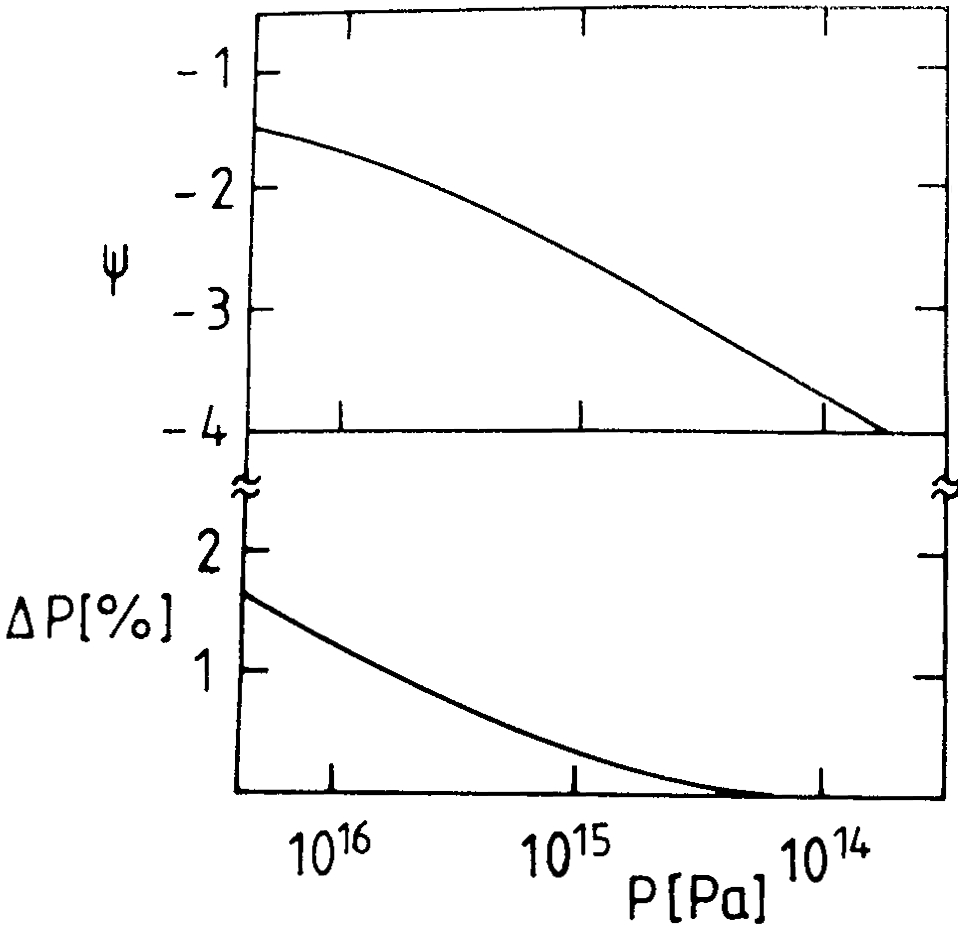
\includegraphics[width=0.9\textwidth,keepaspectratio]{degenpsiP}
\phantomcaption\label{fig:degenelectrocorrection}
\end{subfigure}%
~
\begin{subfigure}[t]{0.5\textwidth}
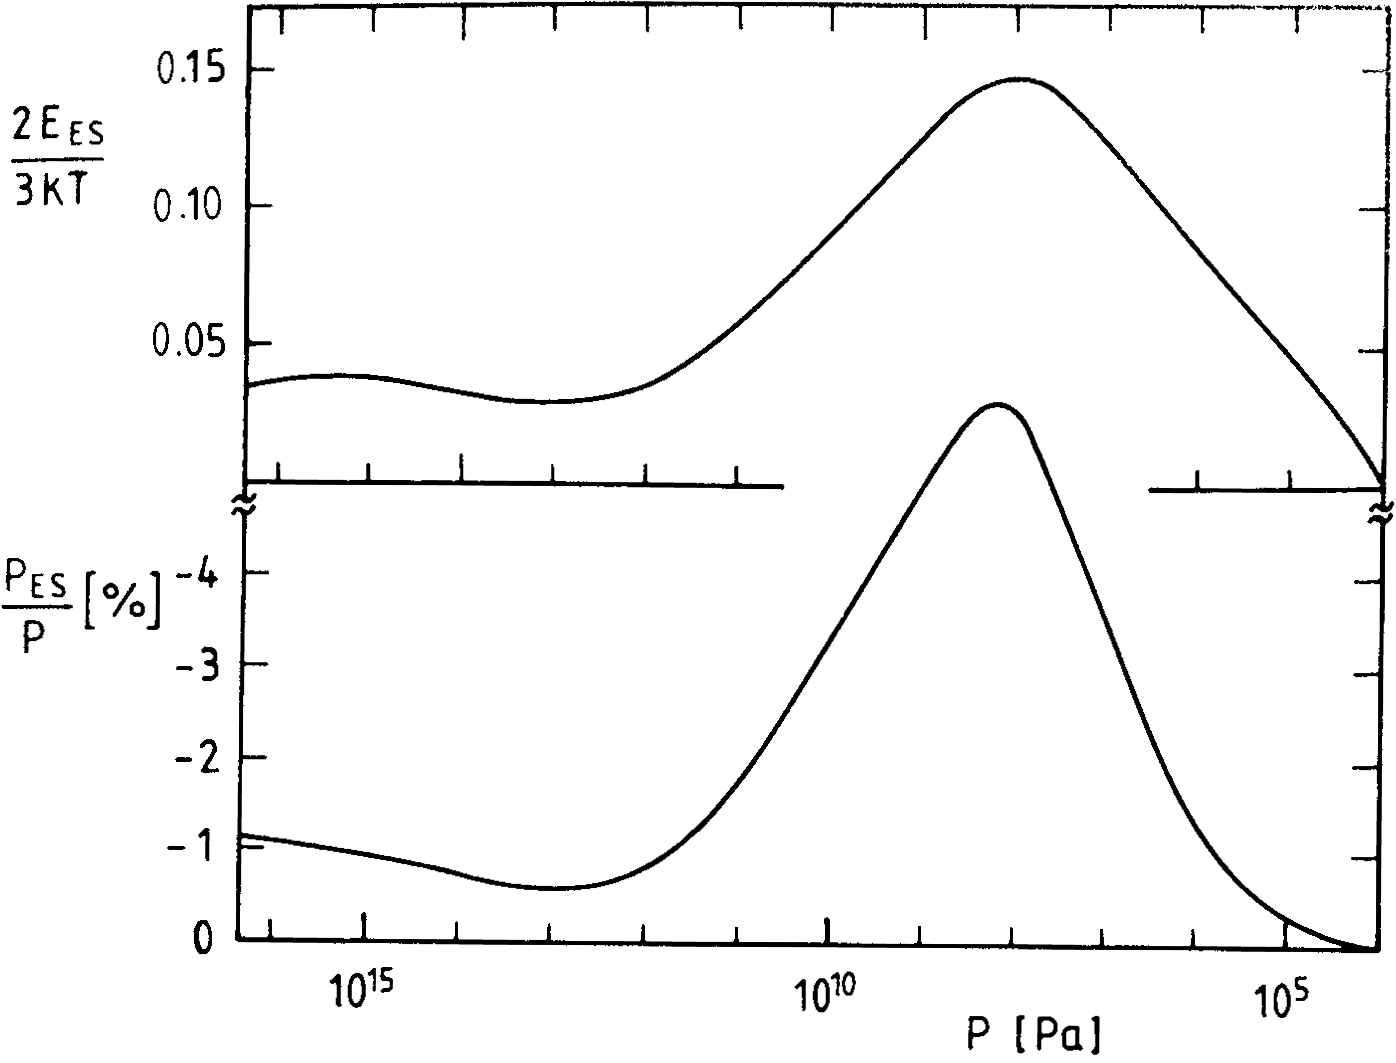
\includegraphics[width=0.9\textwidth,keepaspectratio]{RatioelectroEP}
\phantomcaption\label{fig:RatioelectroEP}
\end{subfigure}
\caption{A sinistra (a): Parametro di degenerazione $\Psi$ e correzioni alla pressione dovute alla degenerazione degli elettroni nell'interno solare. A destra (b): Rapporto fra energia interna traslazionale e coulombiana la prima e fra pressione e correzione coulombiana la seconda. Da \cite{stix91sun}.}
\end{figure}

\'E necessario tenere conto delle deviazioni dalla legge dei gas perfetti:
\begin{itemize}

\item Radiazione. Il contributo alla pressione ed energia interna per unit\'a di volume dei fotoni 
\begin{equation}
P_R=\frac{a}{3}T^4,\ u_R=aT^4
\end{equation}

\item Degenerazione elettronica. Nelle regioni interne del Sole devo tenere conto della degenerazione elettronica, detta $n_e$ la densit\'a numerica, $\psi(P,T)$ il parametro di degenerazione, tale che per $\psi\to-\infty$ si abbia la distribuzione di Boltzmann e per $\psi\to+\infty$ completa degenerazione, e $u_k$ energia cinetica dell'elettrone, si ha:
\begin{equation}
n_e=\rho N_A\frac{1+X}{2}=\intzi{}\frac{8\pi p^2\,dp}{h^3(\exp{\frac{u_k}{KT}-\psi}+1)},\ P_e=\beta P-\rho\gasconstant{}(X+\frac{Y}{4}+\frac{Z}{\exv{A_Z}})=\frac{1}{3}\intzi{}pn_e\TDy{p}{u_k}\,dp
\end{equation}
dove $P-P_R=\beta P$.

\begin{workout}[Parametro di degenerazione: determinazione (prima)]
$u_k$ dipende da $\psi$?
\begin{equation}
u_k=\frac{8\pi}{h^3}\int_0^{\infty}\frac{p^2\epsilon(p)\,dp}{\exp{(-\eta+\midfrac{\epsilon}{KT})}+1}
\end{equation}

\end{workout}

\item Stati legati di nuclei ed elettroni: stati atomici neutri, eccitati e ionizzati.

Per avere una descrizione realistica della ionizzazione in condizioni solare bisogna tener conto delle interazioni non ideali legate alla natura estesa degli atomi.

\end{itemize}

La principale correzione che tiene conto dell'interazioni tra particelle \'e dovuta alle interazioni coulombiane.

\begin{workout}[Correzioni interazioni coulombiane- vedi schermaggio]

\end{workout}

La presenza dello ione $Z_i$ altera la distribuzione di cariche quindi devo determinare il potenziale $\phi_i$ generato da $Z_i$ e dalla distribuzione di cariche attorno: per la formula di Boltzmann, la densit\'a delle particelle con carica Z \'e 
\begin{equation}
n_Z=\overline{n}_Z\exp{-\frac{Ze\phi}{kT}}
\end{equation}
con $\overline{n}_Z$ densit\'a numerica della particell $Z$ in assenza di $Z_i$.

L'equazione di Poisson per $\phi$ \'e
\begin{equation}\label{eq:poissonscreened}
\nabla^2\phi=-4\pi e\sum_Z Zn_Z-4\pi\sum_i Z_i\delta(\vec{r}-\vec{r}_i)
\end{equation}
Nel regime di schermaggio debole, dove l'energia coulombiana \'e molto minore dell'energia termica $e\phi\ll KT$, espando $n_Z$ al prim'ordine quindi in \eqref{eq:poissonscreened} rimane il termine lineare in $\phi$.

Introduco il raggio di Debye:
\begin{equation}
\frac{1}{r_D^2}=\frac{4\pi e^2}{kT}\sum Z^2\overline{n}_Z=\frac{4\pi e^2}{kT}N_A\zeta,\ \zeta=\sum_{i}(Z_i^2+Z_i)\frac{\rho X_i}{A_i}\label{eq:debyeradius}
\end{equation}
quindi dall'equazione \eqref{eq:poissonscreened} ottengo il campo generato dallo ione $Z_i$ in $\vec{r}_i$ a distanza $|\vec{r}-\vec{r}_i|$ come soluzione di:
\begin{equation}\label{eq:poissonspheric}
\frac{r_D^2}{r_i}\TtwoDy{r_i}{(r_i\phi_i)}=\phi_i
\end{equation}
con
\begin{equation}
\phi=\sum_i\phi_i
\end{equation}

\begin{workout}[Raggio di debye e degenerazione elettronica]
Il rapporto fra densit\'a elettronica e quella imperturbata \'e
\begin{equation}
\midfrac{f(\psi-\midfrac{U_e(r)}{KT})}{f(\psi)}
\end{equation}
dove $U_e(r)$ \'e l'energia di interazione di un elettrone
\end{workout}

La soluzione di \eqref{eq:poissonscreened} \'e
\begin{equation}\label{eq:screenedpotential}
\phi_i=\frac{Z_ie}{r_i}\exp{-\midfrac{r}{r_D}}
\end{equation}


\begin{errata}[formula corretta potenziale elettrostatico generato da nuvola elettronica attorno a $Z_i$]

\begin{align}
&\nabla^2V_i=-4\pi e\sum Zn_Z\approx\frac{1}{r_D^2}V_i\intxt{da cui ottengo il potenziale generato dalla nube di cariche attorno a Z}
&\phi_Z=-\frac{eZ}{r_D}
\end{align}
con $r_D$ raggio di Debye definito da:
\begin{equation}
\frac{1}{r_D^2}=\frac{4\pi e^2}{kT}\sum Z^2\overline{n}_Z=\frac{4\pi e^2}{kT}N_A\zeta,\ \zeta=\sum_{i}(Z_i^2+Z_i)\frac{\rho X_i}{A_i}\label{eq:debyeradius}
\end{equation}

\end{errata}

\begin{errata}[correzioni $u_c/P_c$: notazione consistente.]
Le correzioni dovute alle interazioni coulombiane sono
\begin{align}
&u=\frac{3}{2}\frac{\gasconstant{}T}{\mu}+u_c,\ u_c=\frac{1}{2}\sum_ZeZ\overline{n}_Z\phi_Z=-e^3\sqrt{\frac{\pi\rho}{kT}}(N_A\zeta)\expy{\frac{3}{2}}\\
&P=\frac{\rho}{\mu}kT+P_c,\  P_c=\frac{1}{3}u_c
\end{align}
\end{errata}

Le correzioni dovute alle interazioni coulombiane sono
\begin{align}
&u=\frac{3}{2}\frac{\gasconstant{}T}{\mu}+u_c,\ u_c=\frac{1}{2}\int\phi(\vec{r})\rho(\vec{r})\,d^3r\\
&P=\frac{\rho}{\mu}kT+P_c,\  P_c=\frac{1}{3}u_c
\end{align}

La correzione alla pressione dovuta alle interazioni coulombiane raggiunge il picco relativo nelle regioni di ionizzazione parziale di idrogeno ed elio, come illustrato in figura (\subref{fig:RatioelectroEP}).

L'equazione di stato e quindi le grandezze termodinamiche del plasma solare fra cui l'esponente adiabatico $\Gamma_1$, sono principalmente determinate usando lo schema chimico e lo schema fisico: il primo considera atomi e molecole, la cui popolazione per stati eccitati e diversi gradi di ionizzazione \'e ottenuto minimizzando l'energia libera da cui sono ricavate le altre grandezze termodinamiche; utilizzando questo approccio \'e stata ricavata l'equazione di stato MHD. Il secondo considera nuclei ed elettroni come costituenti fondamentali interagenti tramite potenziale Coulombiano e trova le soluzione dell'equazione di Schr\"oedinger per un problema a molti corpi, questo approccio, usato per ricavare l'equazione di stato OPAL, \'e pi\'u adatto per trattare le regioni interne del Sole.

\begin{figure}[!ht]
\begin{subfigure}[b]{0.5\textwidth}
        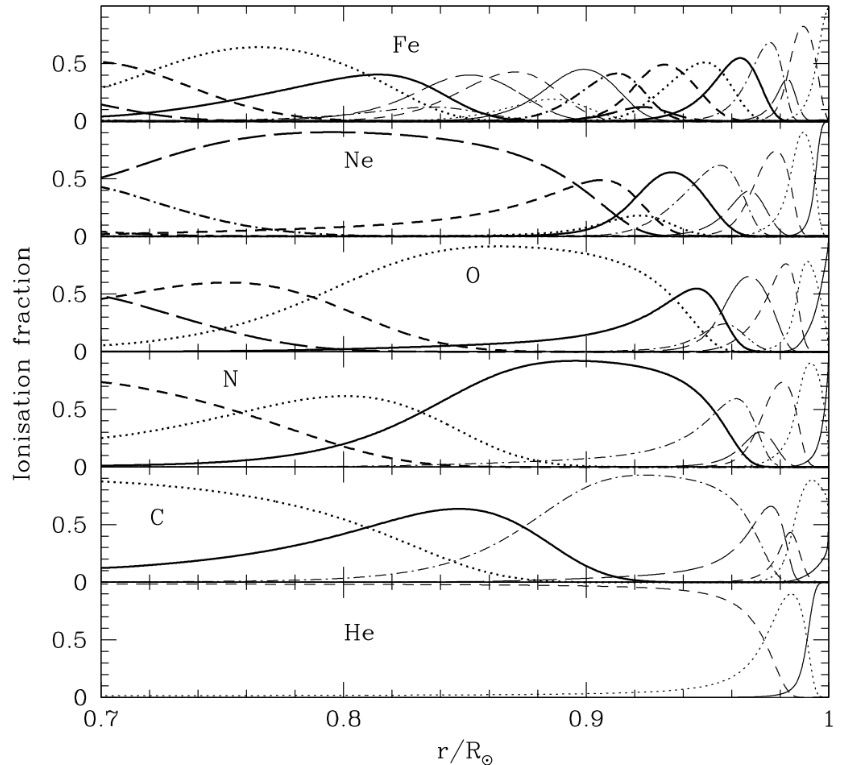
\includegraphics[width=0.9\textwidth,keepaspectratio]{ionfraction}
        \subcaption{Profilo radiale della popolazione dei diversi gradi di ionizzazione per $\cel{He}{4}{}{}$, CNO, $\cel{Ne}{20}{}{}$, $\cel{Fe}{56}{}{}$. Stati di ionizzazione maggiore sono pi\'u interni. Da \cite{basu2008helioseismology}.}\label{ionfraction}
\end{subfigure}%
~
\begin{subfigure}[b]{0.5\textwidth}
        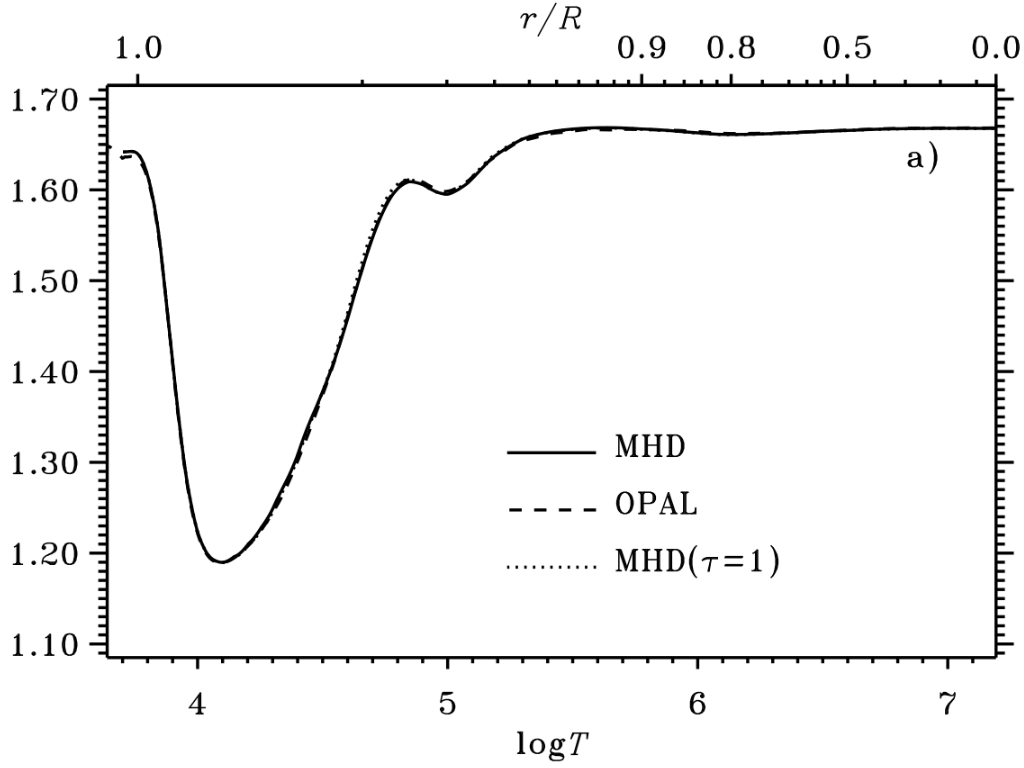
\includegraphics[width=0.9\textwidth,keepaspectratio]{gamma1eos}
        \subcaption{Andamento di $\Gamma_1$ calcolato tramite equazione di stato MHD/OPAL. Da \cite{trampedach2006synoptic}.}\label{fig:gamma1eos}
\end{subfigure}
\end{figure}

Come illustrato in figura (\subref{fig:gamma1eos}), per entrambe $\Gamma_1\approx\midfrac{5}{3}$ nell'interno solare e maggiori deviazioni si hanno nelle regioni di ionizzazione parziale degli elementi in particolare di idrogeno ed elio.

Per stimare l'accuratezza dell'equazione di stata considero la differenza di pressione calcolata usando l'equazione di stato OPAL e MHD:

$\midfrac{\Delta P}{P}\leq1\%$  per $\frac{r}{\rsun{}}\geq0.9$ e $\midfrac{\Delta P}{P}\leq2\permille$ per $\frac{r}{\rsun{}}\leq0.9$, mentre $\midfrac{\Delta \Gamma_1}{\Gamma_1}\leq1\%$  per $\frac{r}{\rsun{}}\geq0.9$ e $\midfrac{\Delta \Gamma_1}{\Gamma_1}\leq1\permille$ per $\frac{r}{\rsun{}}\leq0.9$.

\subsection{Tempo di evoluzione dinamico.}

Per giustificare l'ipotesi di equilibrio idrostatico stimo i tempi caratteristici di evoluzione della struttura solare nel caso la forza dovuta alla pressione o la forza di gravit\'a non fossero bilanciate, approssimando il valore caratteristico della derivata di due variabili con il rapporto del loro valore caratteristico:
\begin{align}
&\tau_{ff}\approx\sqrt{\frac{\rsun{}}{g}}\shortintertext{tempo caratteristico di una distribuzione sferica di materia in caduta libera cio\'e considerando solo il secondo termine in \eqref{eq:motionshell},}
&\tau_{esp}\approx \rsun{}\sqrt{\frac{\rho}{P}}\shortintertext{tempo caratteristico di espansione dovuta al termine di pressione esclusivamente.}\nonumber
\end{align}

Per i valori solari (\ref{wrap-tab:sunO}) $\tau_{ff}\approx\tau_{esp}\approx\SI{27}{\minute}$: quindi la costanza delle caratteristiche solari su tempi molto maggiori giustifica l'ipotesi di equilibrio idrostatico, quindi  riscrivo il tempo scala di evoluzione dinamica come

\begin{equation}
\tau_{idro}^{\odot}= \sqrt{\frac{R^3}{GM}}\approx\frac{1}{2}(G\overline{\rho})\expy{-\frac{1}{2}}
\end{equation}


\section{Conservazione dell'energia.}

La contrazione di una nube di gas interstellare \'e un processo complesso. Quando si raggiunge una configurazione abbastanza densa, tale che il cammino libero medio degli atomi e dei fotoni sia breve, si raggiunge rapidamente l'equilibrio idrostatico e termico locale. Il processo di contrazione gravitazionale continua, su tempi-scala termodinamici, fino a che l'energia prodotta dalle reazioni nucleari bilancia l'energia irradiata.

\subsection{Teorema del viriale}

Il teorema del viriale esprime una propriet\'a statistica di particelle interagenti: si trova una relazione tra energia interna, dovuta al moto traslazionale degli atomi, ed energia potenziale gravitazionale.

L'energia potenziale gravitazionale della stella \'e
\begin{equation}
\Omega=-\int_0^M\frac{Gm(r)}{r}\,dm\label{eq:energiapg}
\end{equation}

Il teorema del viriale dimostra che
\begin{equation}
\frac{1}{2}\TtwoDy{t}{I}=2E_i+\Omega
\end{equation}
con $E_i$ data da \eqref{eq:traslintenergy} e $I=\int r^2\,dm$. In condizioni stazionarie $\frac{1}{2}\TtwoDy{t}{I}\approx0$:
\begin{equation}
0=\int_M\frac{3P}{\rho}\,dm(r)+\Omega
\end{equation}

Detta $W=E_i+\Omega$ l'energia totale della stella, si ha:
\begin{equation}
\Omega=-2E_i\label{eq:virialegpm}
\end{equation}
e dalla conservazione dell'energia $\TDy{t}{W}+L=0$ segue che durante la fase di collasso prima dell'inizio della sequenza principale met\'a dell'energia gravitazionale viene spesa per aumentare l'energia interna e met\'a in luminosit\'a:
\begin{equation}
L=-\frac{1}{2}\dot{\Omega}=\dot{E}_i
\end{equation}

Nel caso in cui la contrazione gravitazionale sia l'unica fonte di energia per una massa gassosa in equilibrio idrostatico, il suo tempo di evoluzione caratteristico \'e il tempo di \kh{}:
\begin{equation}
\tkh{}=\frac{\Omega}{L}\approx\frac{GM^2}{2RL}
\end{equation}
e sostituendo i valori solari di (\ref{wrap-tab:sunO}) si ha $\tkh{}\approx\SI{1.6e7}{\year}$.


\subsection{Conservazione dell'energia interna}

La prima legge della termodinamica esprime la conservazione dell'energia interna, ovvero mette in relazione il flusso di calore $dq$ per unit\'a di massa in un elemento di gas nell'intervallo di tempo $dt$ con la variazione di energia interna per unit\'a di massa $du$ e di volume specifico $dV$:
\begin{equation}
\TDy{t}{q}=\TDy{t}{u}+P\TDof{t}(\frac{1}{\rho})\label{eq:prima}
%\TDy{t}{u}+P\TDy{t}{V}
\end{equation}
che posso riscrivere come
\begin{align}
&\TDy{t}{\ln{T}}=\frac{\Gamma_2-1}{\Gamma_2}\TDy{t}{\ln{P}}+\frac{\TDy{t}{q}}{c_PT}\label{eq:primatemp}\\
&\TDy{t}{\ln{P}}=\Gamma_1\TDy{t}{\ln{\rho}}+\frac{\rho(\Gamma_3-1)}{P}\TDy{t}{q}\label{eq:primapres}
\end{align}
dove ho introdotto gli esponenti adiabatici $\Gamma_i$
\begin{equation}\label{eq:adibatexp}
\Gamma_1=\Dcvar{\TDly{\rho}{P}}{Ad}, \ \Gamma_3-1=\Dcvar{\TDly{\rho}{T}}{Ad},\ \frac{\Gamma_2-1}{\Gamma_2}=\Dcvar{\TDly{P}{T}}{Ad}
\end{equation}

%Il contributo delle modificazioni chimiche aggiungo al lato di destra di \eqref{eq:prima} il termine contenente il potenziale chimico $-\mu_idN_i$ con $\mu_i=\Dcvar{\PDy{N_i}{u}}{S,V}$ all'equilibrio \'e trascurabile.
%Vedi: chemical mixing, equilibrium slowness (partial ionization region, nuclear burning) mass action law: $\sum n_i\mu_i=0$??, minimizzazione energia libera.

Scrivo il bilancio di calore per un elemento di massa unitaria di gas:
\begin{equation}
\TDy{t}{q}=\epsilon-\frac{1}{\rho}\nabla\cdot\vec{F}\label{eq:heatgl}
\end{equation}
dove $\epsilon$ \'e l'energia prodotta per unit\'a di tempo e massa e $\vec{F}$ \'e il flusso di energia verso l'esterno generalmente dovuto alla diffusione di fotoni dalla zona pi\'u calda verso la superficie; sostituendo in \eqref{eq:prima} si ha
\begin{equation}
\TDy{r}{L}=4\pi r^2[\rho\epsilon-\rho\TDof{t}u+\frac{P}{\rho}\TDy{t}{\rho}]\label{eq:fenergyconservation}
\end{equation}

Tengo conto dell'energia generata sotto forma di neutrini, che, alle densit\'a tipiche dell'interno solare, hanno interazioni trascurabili con la materia e quindi dal punto di vista energetico sono paragonabili a un flusso di uscente di cui tengo conto aggiungendo un termine negativo $-\epsilon_{\nu}$ tale che $L_{\nu}=\int_0^M\epsilon_{\nu}\,dm$.

Nel caso stazionario:
\begin{equation}
\TDy{t}{q}=0\ \Rightarrow\ dL=4\pi r^2\rho\epsilon\,dr
\end{equation}
e i processi nucleari che avvengono nella parte centrale forniscono il calore per bilanciare il flusso di energia irradiata.

\section{Diffusione}

La velocit\'a di diffusione relativa di due elementi si pu\'o scrivere:
\begin{align}
&v_{12}=\frac{1}{n_1}\int\,d^3v_1f_1\vec{v}_1-\frac{1}{n_{2}}\int\,d^3v_{2}f_{2}\vec{v}_{2}\\
&=-D_{12}\left[\frac{1}{c_1c_{2}}\PDy{r}{c_1}+\frac{m_{2}-m_1}{c_1m_1+c_{2}m_{2}}\frac{1}{P}\PDy{r}{P}-\frac{m_1m_{2}(\vec{F}_1-\vec{F}_{2})}{KT(c_1m_1+c_{2}m_{2})}+\frac{K_T}{n_1n_{2}}\frac{1}{T}\PDy{r}{T}\right]\label{eq:diffusionaller}
\end{align}
dove ho definito la concentrazione relativa $c_i=\frac{n_i}{n}$, il coefficiente di diffusione $D_{12}=\frac{1}{3}lv_{th}$ con $l\approx(n\sigma)\expy{-1}$ cammino libero medio con $\sigma$ sezione d'urto media e il coefficiente di diffusione termica $K_T$.

%Il primo termine tende a diminuire il gradiente di concentrazione, il secondo del gradiente di pressione, il terzo della forza per unit\'a di massa agente sulle componenti, il quarto del gradiente termico.

L'equazione \eqref{eq:diffusionaller} descrive l'effetto sulle diverse particelle, importante per l'evoluzione chimica solare, delle disomogeneit\'a di composizione, pressione e temperatura presenti nel Sole approssimando la soluzione dell'equazione del trasporto di Boltzmann del trasporto con la distribuzione di equilibrio traslata della velocit\'a di diffusione. La distribuzione di velocit\'a $f_i(\vec{r},\vec{v},t)$ della specie i \'e soluzione dell'equazione del trasporto:
\begin{equation}
\TDy{t}{f_i}=\PDy{t}{f_i}+\vec{v}_i\cdot\PDy{\vec{r}}{f_i}+\vec{F}_i\cdot\PDy{\vec{v}}{f_i}=-\Div_{\vec{p}}(\vec{s})=C(f_j)\label{eq:Btransport}
\end{equation}
$\vec{s}$ \'e il flusso nello spazio dei momenti dovuto alle collisioni. 

Introduco la sezione d'urto collisionale di Rutherford:
\begin{equation}
d\sigma=\frac{4\pi(Z_iZ_j)^2}{\mu^2(\vec{v}-\vec{v}')^4}\frac{d\chi}{\chi^3}
\end{equation}
per piccoli angoli $\chi$ di deviazione della velocit\'a relativa nel sistema CM  e $\mu$ massa ridotta. Considero un parametro d'impatto massimo $\lambda=\max{(r_D,a_0)}$, distanza alla quale il potenziale coulombiano \'e schermato dalle altre cariche:
\begin{equation}
\sigma_{ij}\propto \frac{e^4Z_i^2Z_j^2}{(KT)^2}\ln{\Lambda_{st}}
\end{equation}
da risultati numerici si ha che
\begin{equation}
\ln{\Lambda_{ij}}\propto\ln{[1+0.18769(\frac{4KT\lambda}{Z_iZ_je^2})]}
\end{equation}

Scrivo il termine collisionale $C(f)$, considerando solo il contributo degli urti con la specie j con distribuzione $f_j$ , nella forma
\begin{equation}
C(f_i,f_j)=\int\,d^3p_j\,d\sigma|\vec{v}_i-\vec{v}_j|(f_i'f_j'-f_if_j)
\end{equation}
dove le quantit\'a primate si riferiscono ai valori dopo l'urto. La forza netta dovuta agli urti \'e:
\begin{equation}
\vec{R}_{ij}=\int m\vec{v}C(f_i,f_j)\,d^3v_i\label{eq:friction}
\end{equation}

Considero il problema in cui le due specie hanno velocit\'a relativa media diversa da zero ma piccola rispetto alla velocit\'a termica: nel sistema in cui la prima specie ha velocit\'a media nulla la seconda ha velocit\'a $V_{ij}$ quindi la distribuzione di velocit\'a della prima \'e la distribuzione di equilibrio a temperatura T quella della seconda \'e  la distribuzione di equilibrio a temperatura T traslata di $V_{ij}$, velocit\'a di diffusione:
\begin{equation}
f_j=f_j^{(0)}+\frac{m_j}{KT}(\vec{V}_{ij}\cdot\vec{v}_j)f_j^{(0)}
\end{equation}
da cui si ottiene:
\begin{align}
&\vec{R}_{ij}=n_in_j\mu_{ij}\alpha_{ij}\vec{V}_{ij}\label{eq:resistance}\\
&\alpha_{ij}=\frac{\mu_{ij}}{KT}\int v_r^3\sigma^Tf^{(0)}(\vec{v_r})\,d^3v_r\label{eq:collisionintegral}\\ &\sigma^T=\int(1-\cos{\chi})\,d\sigma\label{eq:sigmatransport}
\end{align}

Nella sedimentazione gravitazionale la forza per unit\'a di volume agente sulle particelle di specie i \'e
\begin{equation}
\vec{F}_i=-\nabla P_i+n_i(q_i\vec{E}+m_i\vec{g})
\end{equation}
e in condizioni di equilibrio il momento trasferito tramite urti con le altre specie \'e uguale alla forza per unit\'a di volume:
\begin{equation}
\vec{F}_i=\sum_{i\neq j}\vec{R}_{ij}%\vec{F}_{ij}=m_{ij}n_in_j\alpha_{ij}\vec{v}_{ij}
\end{equation}

In un plasma costituito da idrogeno, elio ed elettroni per mantenere la neutralit\'a la velocit\'a di diffusione degli elettroni \'e dello stesso ordine di grandezza di quella degli ioni, quindi l'impulso trasferito \'e trascurabile, da cui:
\begin{align}
&F_H\approx F_{HHe}=-\PDy{r}{P_H}+n_H(eE+m_Hg)\\
&F_{He}\approx -F_{HHe}=-\PDy{r}{P_{He}}+n_{He}(2eE+4m_Hg)\\
&E=-\frac{1}{en_e}\PDy{r}{P_e}\intxt{Per le velocit\'a di diffusione si ha}
&v_{HHe}=-\frac{m_{He}T}{m_{HHe}Y\rho \alpha_{HHe}}[\PDy{r}{\ln{(P_eP_H)}}-m_Hg],\ 
n_Hv_H=\frac{(m_{He}n_Hn_{He})}{\rho}v_{HHe}\\
\end{align}

La velocit\'a di diffusione degli elementi pesanti \'e determinata prevalentemente dagli urti con H e He.
Indico con $\eta(A,r)$ la forza per unit\'a di volume sull'elemento di numero atomico Z e di massa A:
\begin{equation}\label{eq:forceperVheavy}
\begin{split}
&\eta(A,r)=-\PDy{r}{P_A}+n_A(Z_Ae\vec{E}+Am_H\vec{g})\\
&=-n_Ak_BT(\PDy{r}{\ln{P_A}}+Z_A\PDy{r}{\ln{P_e}}+\frac{AGm_HM}{r^2k_BT})
\end{split}
\end{equation}

In condizioni stazionarie si ha:
\begin{equation}\label{eq:diffheavystatinary}
\vec{F}_A\approx\vec{R}_{A,H}+\vec{R}_{A,He}=\eta(A,r)
\end{equation}
e poich\'e
\begin{equation}
\frac{\eta(A,r)}{n_Av_H(m_{A,H}n_H\alpha_{A,H})}\propto\frac{1}{XZ_A}
\end{equation}
posso trascurare $\eta(A,r)$ in \eqref{eq:diffheavystatinary} ed esplicitando i contributi $R_{A,H}$ e $R_{A,He}$
ottengo
\begin{equation}\label{eq:diffvelocityA}
v_A(1+2\frac{Y}{X})\approx-v_H
\end{equation}
%&n_Av_A(m_{AH}n_Hw_{AH})(1+2\frac{Y}{X})\approx-n_Av_H(m_{AH}n_Hw_{AH})

\begin{workout}[Velocit\'a sedimentazione ioni pesanti]

Il flusso di elementi pesanti $n_Av_A$ \'e determinato dalle collisioni degli ioni pesanti con  H e He:

\begin{align}
&\vec{R}_{A,H}=m_{A,H}n_An_Hw_{A,H}(\vec{v}_a-\vec{v}_H)\intxt{and similar equation for collision with He. La condizione di equilibrio \'e:}
&\vec{F}_A\approx\vec{R}_{A,H}+\vec{R}_{A,He}=\eta(A,r)\intxt{con}
&\eta(A,r)=-\PDy{r}{P_A}+n_A(Z_Ae\vec{E}+Am_H\vec{g})=-n_Ak_BT(\PDy{r}{\ln{P_A}}+Z_A\PDy{r}{\ln{P_e}}+\frac{AGm_HM}{r^2k_BT})\\
&\vec{R}_{A,H}=m_{A,H}n_An_H\alpha_{A,H}(\vec{v}_A-\vec{v}_H)\\
&\vec{R}_{A,He}=m_{A,He}n_An_{He}\alpha_{A,He}(\vec{v}_A-\vec{v}_{He})\\
&n_Av_A(m_{A,H}n_H\alpha_{A,H})(1+2\frac{Y}{X})=-n_Av_H(m_{A,H}n_H\alpha_{A,H})+\eta(A,r)\\
&\frac{\eta(A,r)}{n_Av_H(m_{A,H}n_H\alpha_{A,H})}\propto\frac{1}{XZ_A}\intxt{quindi approssimativamente si ha:}
&v_A(1+2\frac{Y}{X})=-v_H
\end{align}

\end{workout}

La diffusione termica concentra le particelle pi\'u pesanti (e pi\'u cariche) nelle zone pi\'u calde: in presenza di un gradiente termico si ha un trasferimento netto di momento negli urti in direzione del gradiente, in \eqref{eq:friction}, dovuto al maggior numero di particelle energetiche provenienti dalle regioni pi\'u calde, ci\'o \'e dovuto alla dipendenz della sezione d'urto coulombiana dalla velocit\'a relativa $\propto v\expy{-4}$ (probabilit\'a di collisione $\propto v\expy{-3}$).


\begin{workout}[Diffusione termica]
Vedi Roussel-Dupr\'e: computations of ion diffusion coefficients from the Boltzmann-Fokker-Plank equation.

Per un gas a pressione e composizione omogenea scrivo la distribuzione di una specie di particelle tramite un espansione al primo ardine in $\tau$, tempo fra collisioni
%\begin{comment}
\begin{align}
&f=f^{(0)}-KT(\vec{v}\tau\nabla T)\PDof{T}(\frac{f^{(0)}}{KT})=f^{(0)}-\frac{2\lambda}{5Kn_1}(\vec{v}\nabla T)\PDof{T}(\frac{m_1f^{(0)}}{KT})&\intxt{Il momento trasferito per unit\'a di volume tra due specie diverse in presenza di un gradiente termico, a causa degli urti, \'e}\\
&\vec{P}=n_1n_2\int\int f_1f_2m_{12}\vec{g}\nu(g)\,d^3v_1\,d^3v_2=\frac{2m_{12}}{5K(m_1+m_1)}\PDy{T}{\bar{\nu}}(n_2m_2\lambda_1-n_1m_1\lambda_2)\nabla T\\
&\overline{\nu}=\frac{1}{3}\int f^{(0)}\frac{m_{12}g^2}{kT}\nu(g)\,d^3g\\
&\vec{v}_{HHe}^{th}\approx\frac{2}{5kN_Hn_{He}}(\frac{n_{He}m_{He}\vec{q}_H-n_Hm_H\vec{q}_{He}}{m_H+m_{He}})\PDy{T}{\ln{\overline{\nu}}}
\end{align}
%end{comment}


Considero da prima un plasma di \Pelectron e \Pproton; per effetto della dipendenza della frequenza di collisione dalla velocit\'a relativa delle particelle si ha una forza per unit\'a di volume che modifica il campo elettrico:
\begin{equation}
P_{HHe_{th}}=\alpha_{HHe}n_Hn_{He}\frac{T}{P}\nabla T
\end{equation}
Si tiene conto del flusso di massa, momento ed energia nelle equazioni di conservazione attraverso le equazioni sviluppate da Burgers (1969).

\end{workout}

\begin{minipage}{\linewidth}
\begin{tikzpicture}
\node[inner sep=0pt] (image) at (0,0)
  {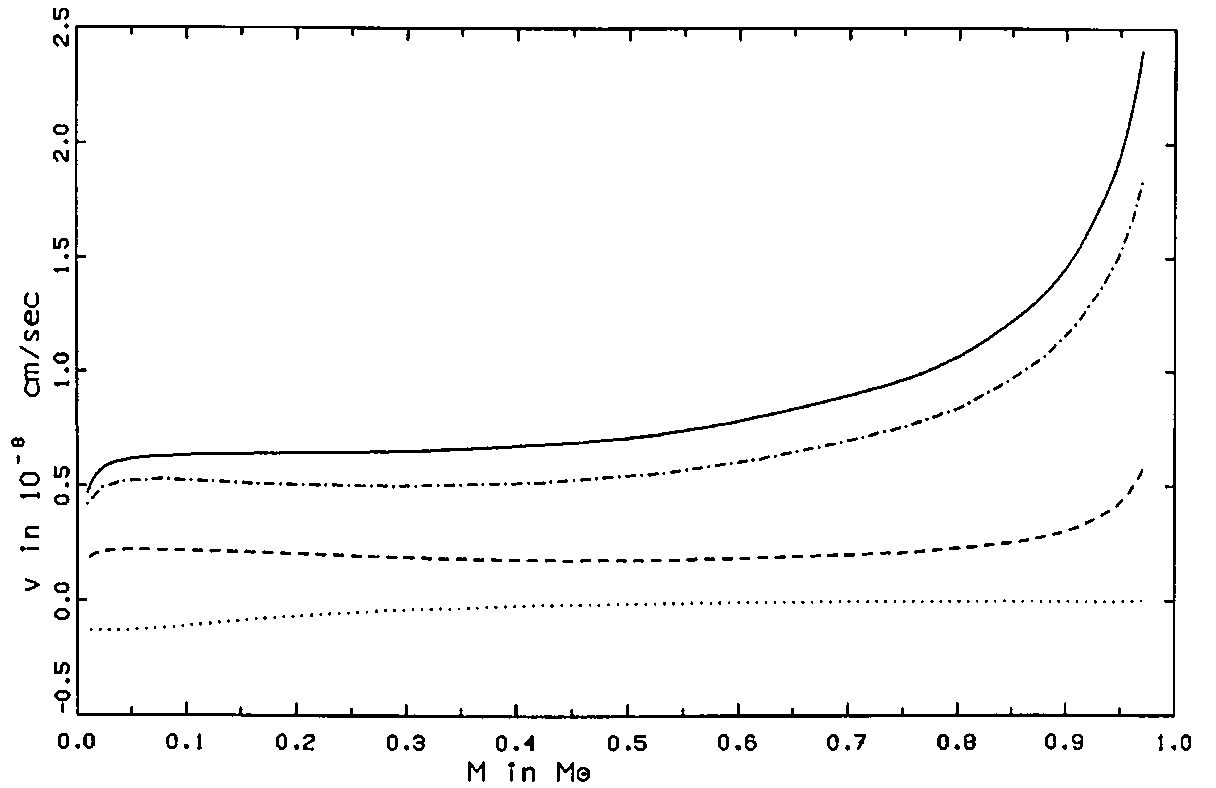
\includegraphics[keepaspectratio=true,width=0.5\textwidth]{Hdiffusion}};
  \draw [thick,dotted] (-3.4,1.5) -- (-3,1.5) node[right] {$\propto\nabla c$};
 \draw [thick,dashed] (-3.4,1.9) -- (-3,1.9) node[right] {$\propto\nabla T$};
    \draw [thick,dash dot] (-3.4,2.3) -- (-3,2.3) node[right] {$\propto\nabla P$};
    \node (caption) at (8.5,-2.5) { \begin{minipage}[c]{0.48\textwidth}
\captionof{figure}{Contributi alla velocit\'a di diffusione di H-He in modello solare. Da \cite{wam88hydrogen}.}%   
    \end{minipage}};
\node[] (massconsdiff) at (8.5,1) {\begin{minipage}[c]{0.48\textwidth}

Sebbene il tempo caratteristico per percorre un raggio solare sia lungo $\tau_{diff}\approx\SI{6e13}{\year}$ i processi di diffusione producono effetti non trascurabili sulla struttura solare e sull'abbondanza superficiale degli elementi: la loro inclusione nei \mss{} produce un miglior accordo con le osservazioni.

\end{minipage}
};
\end{tikzpicture}
\end{minipage}

{\let\clearpage\relax\let\cleardoublepage\relax
\chapter{Trasporto dell'energia}
}

\section{Trasporto radiativo.}

Nell'interno stellare il cammino libero medio dei fotoni \'e molto corto $\frac{1}{\kappa\rho}\approx\SI{1}{\cm}\ll \rsun{}$, con $\kappa$ opacit\'a radiativa per unit\'a di massa, quindi considero la radiazione localmente in equilibrio con la materia. Il flusso di energia verso la superficie \'e generato da una piccola anisotropia nell'intensit\'a descritta al prim'ordine tramite:
\begin{equation}
I_{\nu}=B(\nu,T)-\frac{1}{\kappa_{\nu}'\rho}\nabla_s B(\nu,T)
\end{equation}
integrando sull'angolo solido, il flusso di energia risulta
\begin{align}
&\vec{F}_{\nu}=-\frac{4\pi}{3\kappa_{\nu}\rho}\nabla B(\nu,T)\shortintertext{ed esplicitando il gradiente termico e integrando sulle frequenze}
&\vec{F}=-[\frac{4\pi}{3\rho}\intzi{}\frac{1}{\kappa_{\nu}}\PDy{T}{B(\nu,T)}\,d\nu]\nabla T\label{eq:radiativeflux}
\end{align}

Definisco l'opacit\'a media di Rosseland:
\begin{equation}
\frac{1}{\kappa}=(\intzi{}\PDy{T}{B(\nu,T)})\expy{-1}\intzi{}\,d\nu\frac{1}{\kappa_{\nu}}\PDy{T}{B(\nu,T)}=(\frac{acT^3}{\pi})\expy{-1}\intzi{}\,d\nu\frac{1}{\kappa_{\nu}}\PDy{T}{B(\nu,T)}\label{eq:rosselandopacity}
\end{equation}
quindi riscrivo \eqref{eq:radiativeflux} utilizzando la pressione di radiazione $P_{rad}=\int\,d\nu\frac{4\pi}{3c}B_{\nu}=\frac{1}{3}aT^4$:
\begin{align}
&\vec{F}=-\frac{4\pi}{3\kappa\rho}\nabla B=-\frac{4\pi}{3\kappa\rho}\nabla B=-\frac{c}{\kappa\rho}\nabla P_{rad}\shortintertext{che per una distribuzione sferica di materia diventa}
&F_r=-\frac{c}{\kappa\rho}\TDof{r}(\frac{1}{3}aT^4)=-\frac{4acT^3}{3\kappa\rho}\TDy{r}{T}\label{eq:radfluxTgradrelation}
\end{align}

Definisco il gradiente radiativo a partire da \eqref{eq:radfluxTgradrelation}
\begin{equation}
\nrad{}=\Dcvar{\PDly{P}{T}}{rad}=\frac{3}{16\pi acG}\frac{\kappa l(r)P}{m(r)T^4}\label{eq:radiativegradient}
\end{equation}
con $l(r)=4\pi r^2F$ luminosit\'a totale in funzione di r.

\subsection{Opacit\'a.}

I fenomeni che contribuiscono all'opacit\'a nel Sole sono:

\begin{itemize}

\item \parbox[t]{\dimexpr\textwidth-\leftmargin}{%
\vspace{-2.5mm}
\begin{wrapfigure}{r}{0.5\textwidth}
\centering
\vspace{-\baselineskip}
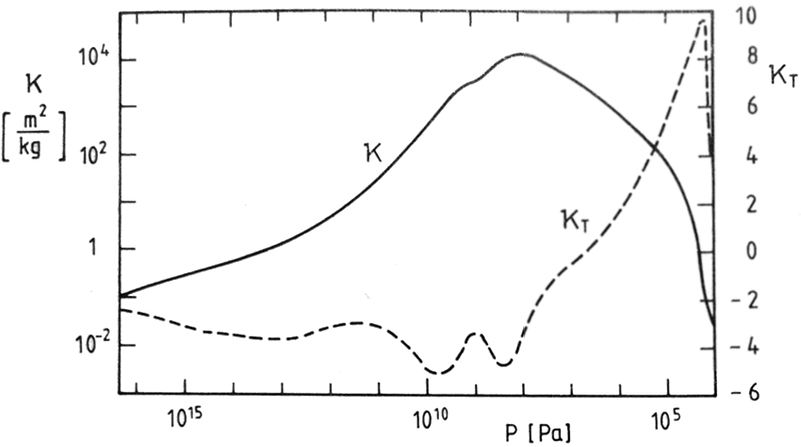
\includegraphics[keepaspectratio,width=0.9\linewidth]{opacitylld}
\caption{Profilo radiale di $\kappa$ e $\PDly{T}{\kappa}$. Da \cite{stix91sun}.}
\end{wrapfigure}


Scattering fotone-elettrone (sc). Classicamente \'e descritto come lo scattering di un'onda elettromagnetica piana da parte di un dipolo oscillante, scattering Thomson per $h\nu\ll m_ec^2$

\begin{align}
&\kappa_{\nu}\propto\frac{r_e^2}{\mu_em_u}, \kappa_{sc}=0.20(1+X)\si{\squared\cm\per\gram}\\
&r_e=\SI{2.82e-13}{\cm}
\end{align}

Per $T\geq\SI{e8}{\kelvin}$ il momento trasferito all'elettrone non \'e trascurabile, scattering Compton.

}

\item Brehmstrahlung inverso (ff). L'assorbimento di un fotone da parte di un elettrone libero \'e energeticamente possibile quando l'elettrone \'e vicino ad uno ione, l'opacit\'a in questo caso ha l'andamento

\begin{equation}
\kappa_{ff}\propto\rho T\expy{-\frac{7}{2}}
\end{equation}

si tiene conto degli effetti quantistici tramite un opportuno coefficiente, il fattore di Gaunt.

\item Reazioni di ionizzazione (bf).

\item Transizione elettronica a livelli eccitati (bb).

\item Scattering atomici e ione $H^-$. La presenza di metalli con potenziale di ionizzazione minore di H ed He rendono disponibile elettroni per la formazione di $H^-$, sistema debolmente legato per cui un fotone con $h\nu>\SI{0.75}{\ev}$ o $\lambda<\SI{1655}{\nano\meter}$ pu\'o essere assorbito.

\end{itemize}

La conduzione pu\'o essere trascurata in quanto nel Sole $l_{\Pphoton}\gg l_{\Pelectron}$, cio\'e i tempi caratteristici per il trasporto di calore per conduzione sono molto maggiori di quelli radiativi.

%\begin{equation}
%\delta\kappa(r)=\frac{\kappa_{OPAL}(\bar{T}(r),\bar{\rho}(r),\bar{Y}(r),\bar{Z}(r))}{\kappa_{OP}(\bar{T}(r),\bar{\rho}(r),\bar{Y}(r),\bar{Z}(r))}-1\leq0.025
%\end{equation}

\begin{tikzpicture}[]
%([shift={(1.5,0)}]0,0)

\node[anchor=north west] (opint) at (0,0) {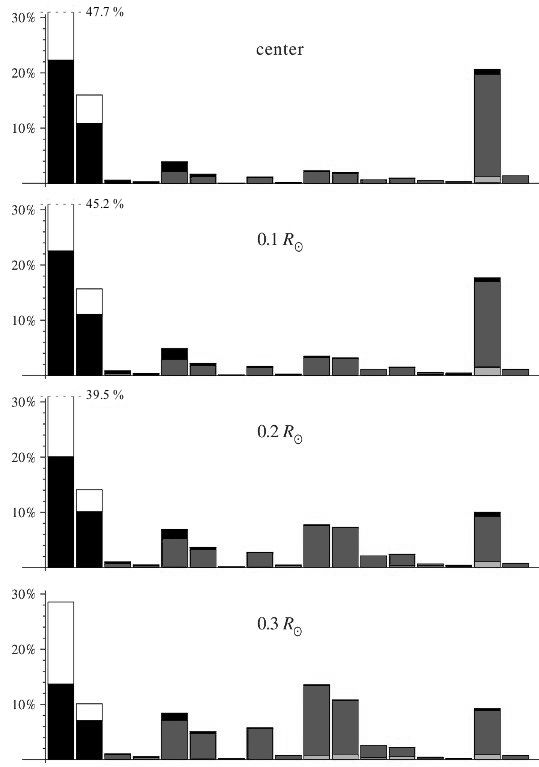
\includegraphics[height=0.35\textheight,keepaspectratio]{opcontrib-int-g}};
\node[anchor=west,right=2.5cm of opint.east] (opout) {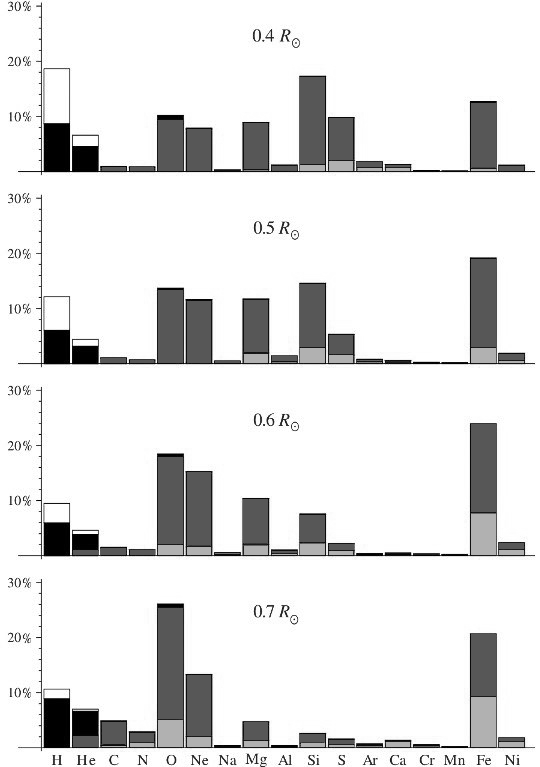
\includegraphics[height=0.35\textheight,keepaspectratio]{opcontrib-out-g}};
\begin{scope}[scale=0.6]
\node[draw,anchor=west,label={[label distance=2mm]-90:Scattering \Pphoton\Pelectron},minimum size=5mm,below right=1cm and 9mm of opint.east] (sc) {};
\node[draw,label={[label distance=2mm]-90:ff},fill=black,minimum size=5mm,above=10mm of sc] (ff) {};
\node[draw,label={[label distance=2mm]-90:bb},fill=bb,minimum size=5mm,above=10mm of ff] (bb) {};
\node[draw,label={[label distance=2mm]-90:bf},fill=bf,minimum size=5mm,above=10mm of bb] (bf) {};
\end{scope}

\begin{scope}[node distance=3.62mm]
\node[minimum size=2mm,name=hydrogen, right=6.5mm of opint.south west] {\tiny H};
\node[minimum size=2mm,name=helium, right=of hydrogen.west] {\tiny He};
\node[minimum size=2mm,name=carbonium, right=of helium.west] {\tiny C};
\node[minimum size=2mm,name=nitrum, right=of carbonium.west] {\tiny N};
\node[minimum size=2mm,name=oxygen, right=of nitrum.west] {\tiny O};
\node[minimum size=2mm,name=neon, right=of oxygen.west] {\tiny Ne};
\node[minimum size=2mm,name=sodium, right=of neon.west] {\tiny Na};
\node[minimum size=2mm,name=magnesium, right=of sodium.west] {\tiny Mg};
\node[minimum size=2mm,name=alluminium, right=of magnesium.west] {\tiny Al};
\node[minimum size=2mm,name=silicium, right=of alluminium.west] {\tiny Si};
\node[minimum size=2mm,name=sulfur, right=of silicium.west] {\tiny S};
\node[minimum size=2mm,name=argon, right=of sulfur.west] {\tiny Ar};
\node[minimum size=2mm,name=calcium, right=of argon.west] {\tiny Ca};
\node[minimum size=2mm,name=cromum, right=of calcium.west] {\tiny Cr};
\node[minimum size=2mm,name=manganese, right=of cromum.west] {\tiny Mn};
\node[minimum size=2mm,name=ferrum, right=of manganese.west] {\tiny Fe};
\node[minimum size=2mm,name=nikel, right=of ferrum.west] {\tiny Ni};

\end{scope}
 
\node[anchor=north west, below right=1mm and 0.5cm of opint.south west] {\parbox{\textwidth}{\captionof{figure}{Importanza dei varii contributi all'opacit\'a nell'interno solare; composizione GS98. Da \cite{bla11opacity}.}\label{fig:opacitycontrib} }};
 
\end{tikzpicture}


\section{Condizione di in-stabilit\'a dinamica: trasporto convettivo.}

Una regione stellare \'e convettivamente stabile se una perturbazione di densit\'a infinitesima non cresce ad ampiezza finita. Considero l'equazione del moto per blob di materia che subisce spostamento $\Delta r$ dalla  posizione di equilibrio:
\begin{equation}
\rho\PtwoDy{t}{(\Delta r)}=-g\Delta\rho=-g[\Dcvar{\TDy{r}{\rho}}{e}-\Dcvar{\TDy{r}{\rho}}{amb}]\Delta r
\end{equation}

La forza di archimede ha verso opposta alla perturbazione se $[\Dcvar{\TDy{r}{\rho}}{e}-\Dcvar{\TDy{r}{\rho}}{amb}]>0$ .

Considero un'equazione di stato generica $\rho(P,T,\mu)$ e definita tramite:
\begin{align}
&\frac{d\rho}{\rho}=\alpha\frac{dP}{P}-\delta\frac{dT}{T}+\phi\frac{d\mu}{\mu}\label{eq:deltatherm}\\
&P=\frac{\rho\gasconstant{}T}{\mu}\quad\Rightarrow\quad\alpha=\delta=\phi=1
\end{align}

Definisco le lunghezze caratteristiche per variazione di densit\'a e pressione:
\begin{equation}
\densityscale{}=-\frac{dr}{d\ln{\rho}},\ H_P=-\frac{dr}{d\ln{P}}
\end{equation}
e i gradienti termici per il blob, l'ambiente e il gradiente di composizione chimica ambientale
\begin{equation}
\nabla=\Dcvar{\TDly{P}{T}}{amb},\ \nabla_e=\Dcvar{\TDly{P}{T}}{blob},\ \nmu{}=\Dcvar{\TDly{P}{\mu}}{amb}\label{eq:nablavitense}
\end{equation}

Riscrivo l'equazione del moto utilizzando l'equazione di stato, supponendo il moto dell'elemento in equilibrio di pressione con l'ambiente, essendo $\nmu{}_{blob}\approx0$:
\begin{equation}
\PtwoDy{t}{(\Delta r)}=-g\frac{\delta}{H_P}[\nabla_e-\nabla-\frac{\phi}{\delta}\nmu{}]\Delta r\label{eq:galleggiamento}
\end{equation}
suppongo inoltre un moto del blob adiabatico $\nabla_e=\nabla_{ad}$ con
\begin{equation}
\nabla_{ad}=\frac{P\delta}{T\rho c_P}
\end{equation}

Introduco la frequenza di \bv{}:
\begin{equation}
N^2=g(\frac{1}{\Gamma_1P}\TDy{r}{P}-\frac{1}{\rho}\TDy{r}{\rho})=g(\frac{1}{\densityscale{}}-\frac{g}{c_s^2})\label{eq:bvfs}
\end{equation}
$N^2$ rappresenta la massima frequenza sotto cui pu\'o oscillare una particella di fluido sottoposta a onde di gravit\'a mantenendo l'equilibrio di pressione con l'ambiente.

Riscrivo l'equazione \eqref{eq:galleggiamento}
\begin{equation}
\PtwoDy{t}{(\Delta r)}=-N^2\Delta r
\end{equation}
che descrive un comportamento oscillatorio per $N^2>0$, cio\'e una regione solare \'e stabile per convezione se

\begin{equation}
\nrad{}<\nad+\frac{\phi}{\delta}\nmu{}\label{eq:ledoux}
\end{equation}

dove ho usato $\nabla_{amb}=\nrad{}$ definito in \eqref{eq:radiativegradient}, cio\'e il gradiente che si ha nel caso la luminosit\'a si trasportata dai fotoni; nelle zone in cui il criterio di Ledoux (o \sch{} se trascuro il gradiente di $\mu$) non \'e verificato si ha trasporto convettivo.

Le stelle con massa $M\leq1.1\msun{}$ hanno una regione radiativa interna mentre la parte esterna \'e convettiva: la regione in cui vale l'uguaglianza in \eqref{eq:ledoux} \'e la base della zona convettiva, la cui posizione \'e determinata dall'aumentare dell'opacit\'a col diminuire della temperatura.
% e dal gradiente adiabatico, il cui valore \'e diminuito dal calore latente di idrogeno ed elio nelle regioni di ionizzazione parziale.

Una maggiore efficienza del trasporto convettivo di energia si riflette in una minore differenza tra il gradiente di temperature adiabatico ed effettivo.

\begin{figure}[!h]
\begin{subfigure}[b]{0.55\textwidth}
    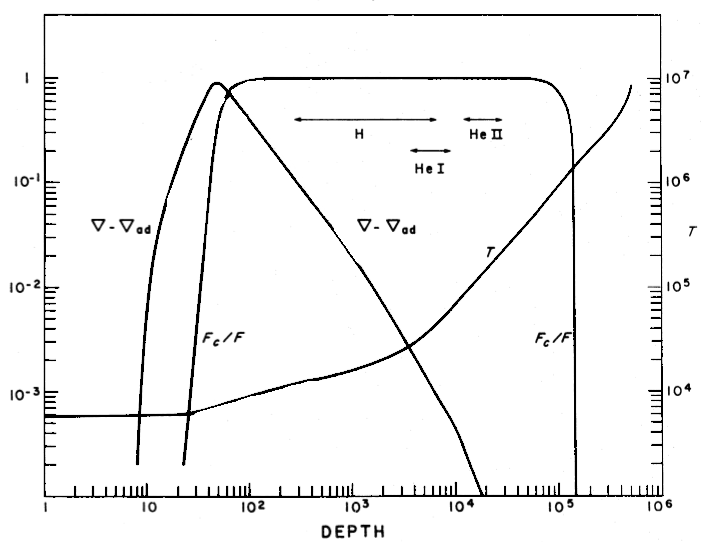
\includegraphics[ width=0.99\textwidth,keepaspectratio]{proportionflux}
    \subcaption{Profilo radiale (profondit\'a in \si{\kilo\meter}) del flusso convettivo $F_c$ rispetto al flusso totale $F$, della super-adiabaticit\'a $\nabla-\nad{}$ e regioni di ionizzazione idrogeno e $\cel{He}{4}{}{}$. Da \cite{gou76convection}.}
    \label{fluxproportion}
\end{subfigure}
~
\begin{subfigure}[b]{0.4\textwidth}
\centering
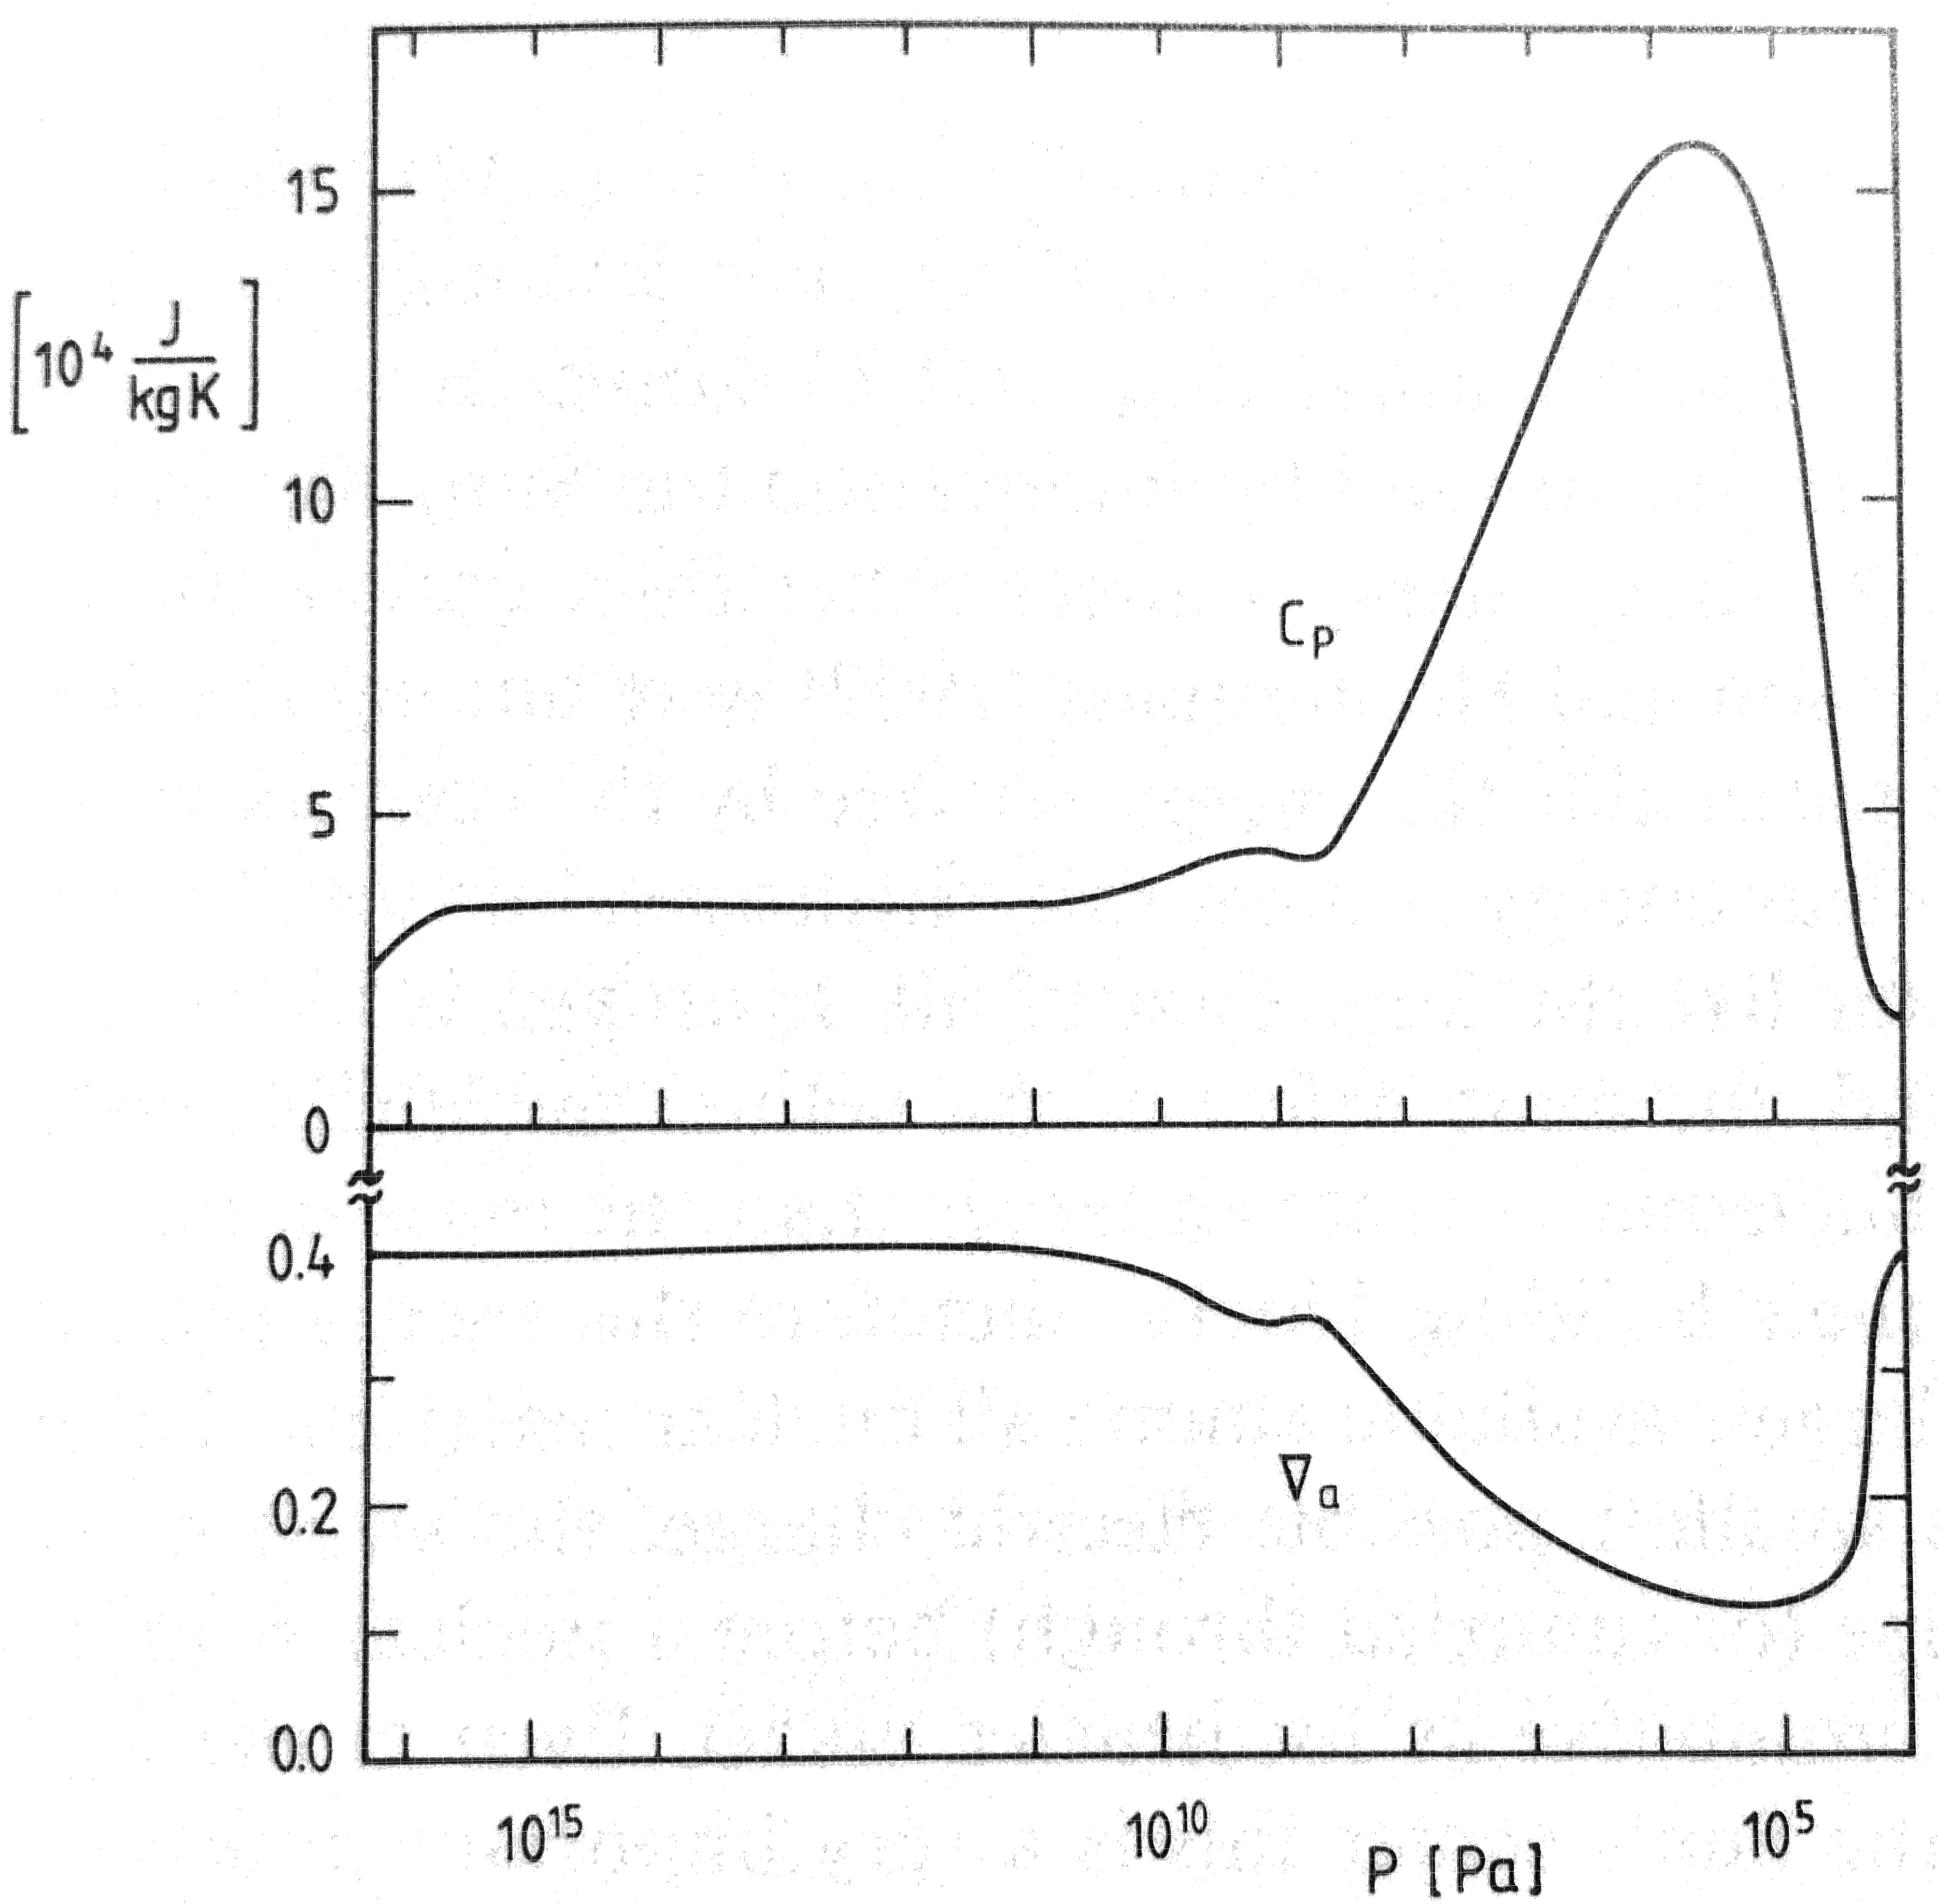
\includegraphics[keepaspectratio,width=0.9\textwidth]{specificheatnablaa}
\subcaption{Profilo radiale di $c_P$ e $\nabla_a$: si ha cambiamento di comportamento nelle regioni di ionizzazione parziale di idrogeno ed elio. Da \cite{stix91sun}.}
\end{subfigure}
\end{figure}


\subsection{Teoria della mixing-length.}

In presenza di convezione il flusso di energia verso l'esterno ha una componente radiativa, determinata dal gradiente di temperatura, e una componente dominante convettiva 
\begin{equation}
F=F_{con}+F_{rad}=\frac{\lsun{}}{4\pi r^2}
\end{equation}
Definisco il gradiente radiativo fittizio:
\begin{equation}
F=\frac{4acG}{3}\frac{T^4m}{\kappa Pr^2}\nrad{}\label{eq:fictionrad}
\end{equation}

Per determinare il gradiente di temperatura effettivo $\nabla$ uso la teoria della mixing-length (\cite{prandtl25tur} e \cite{vitense53kon}):
si considera l'eccesso di calore trasportato dai blob di gas nel moto convettivo $c_P\Delta T$ rispetto all'ambiente, il cui cammino libero medio \'e la mixing-length $l_m=\alpha H_P$, che da luogo al flusso di energia

\begin{equation}
F_{con}=\exv{\rho vc_P\Delta T}\label{eq:convectiveflux}
\end{equation}

dove $\exv{}$ indica una media opportuna sulla sfera di raggio r. Determino il valor medio della differenza di temperatura prendendo come valore caratteristico dello spostamento del blob, considerando moti in entrambi i versi, $\Delta r\approx\frac{l_m}{2}$:
\begin{equation}
\frac{\Delta T}{T}\approx\frac{1}{T}\PDy{r}{(\Delta T)}\frac{l_m}{2}=(\nabla-\nabla_e)\frac{l_m}{2}\frac{1}{H_P}
\end{equation}

Assumo il lavoro medio fatto dalla forza di galleggiamento per unit\'a di massa $-g\frac{\Delta\rho}{\rho}$ uguale al valore medio della forza, cio\'e la met\'a di quello alla superficie sferica data, moltiplicato lo spostamento medio $\frac{l_m}{2}$ quindi, assumendo in oltre che in media met\'a del lavoro fatto dalla forza di galleggiamento sia trasformato in energia cinetica del blob si ottiene

\begin{equation}
v^2=g\delta(\nabla-\nabla_e)\frac{l_m^2}{8H_P}\label{eq:blobvelocity}
\end{equation}

Infine determino gli scambi radiative del blob: il modulo del flusso radiativo \'e proporzionale al gradiente termico in direzione normale alla superficie del blob
\begin{equation}
f=\frac{4acT^3}{3\kappa\rho}|\PDy{n}{T}|
\end{equation}
quindi l'energia scambiata dall'intera superficie S del blob \'e $\lambda=Sf$ che determina, per la prima legge della termodinamica, una variazione di temperatura per unit\'a di tempo:
\begin{equation}
\PDy{t}{T_e}=-\frac{\lambda}{\rho Vc_P}
\end{equation}
indicato con $V$ il volume del blob.

La variazione della temperatura del blob per unit\'a distanza percorsa \'e quindi
\begin{equation}
\Dcvar{\TDy{r}{T}}{e}=\Dcvar{\TDy{r}{T}}{ad}-\frac{\lambda}{\rho Vc_Pv}\label{eq:Tchangelength}
\end{equation}
e approssimando il gradiente normale alla superficie con $\exv{\Delta T}$ ed usando le definizioni \eqref{eq:nablavitense} si ottiene:
\begin{equation}
\frac{\nabla_e-\nad{}}{\nabla-\nabla_e}=\frac{6acT^3}{\kappa\rho^2c_Pl_mv}
\end{equation}

Le 5 equazioni \eqref{eq:fictionrad},\eqref{eq:radiativegradient}, \eqref{eq:convectiveflux}, \eqref{eq:blobvelocity}, \eqref{eq:nablavitense} determinano completamente le variabili $F_{rad}, F_{con}, v, \nabla_e, \nabla$ in funzione di $P,T,l(r),m(r),c_P,\nad{},\nrad{},g$ .


{\let\clearpage\relax\let\cleardoublepage\relax
\chapter{Produzione di energia: reazioni di fusione.}
}

Il tempo trascorso da una stella di massa solare in sequenza principale considerando \'e il tempo necessario per la massa di idrogeno nel core di fusione (le temperature necessarie perch\'e il rate di reazione sia apprezzabile si raggiungono nella regione pi\'u interna che costituisce una frazione $f$ pari al $15\%$ della massa solare) ad esaurirsi:

\begin{equation}
\tau_n\approx\frac{E_n}{L}=\frac{fX\msun Q}{\lsun}\approx\SI{e+10}{\year},\ Q\approx\SI{6.3e18}{\erg\per\gram}
\end{equation}

L'energia liberata dalle reazioni nucleari per grammo per secondo $\epsilon(\rho,T,X_i)$ \'e determinata dalla probabilit\'a che la reazione $X(a,b)Y$ abbia luogo. Sia $E$ l'energia cinetica nel centro di massa dei nuclei, la sezione d'urto $\sigma(E)$ di fusione \'e:
\begin{equation}
\sigma(E)=\pi\lambdabar^2P_0(E)S(E)
\end{equation}

La lunghezza d'onda di de Broglie relativa delle particelle descrive l'indeterminazione sulla posizione nell'urto di due particelle con momento relativo p:
\begin{equation}
\lambdabar=\frac{\hbar}{p}=\frac{\hbar}{\sqrt{2mE}}
\end{equation}

Il fattore astrofisico $S(E)$ descrive l'interazione tra i due reagenti a livello nucleare ed \'e debolmente dipendente dall'energia lontano da risonanze.

La probabilit\'a di attraversamento della barriera coulombiana \'e:
\begin{equation}
P_0(E)=\exp{-2\pi\eta},\ \eta=\sqrt{\frac{m}{2}}\frac{Z_1Z_2e^2}{\hbar E\expy{\frac{1}{2}}}
\end{equation}
Scrivo la sezione d'urto per i nuclei di carica $Z_1$, $Z_2$ e m massa ridotta:
\begin{equation}
\sigma(E)=\frac{S(E)}{E}\exp{-2\pi\eta}\label{eq:fusioncrosssection}
\end{equation}

La funzione $\epsilon(\rho,T,X_i)$ \'e determinata dalla somma di tutti i contributi
\begin{equation}
\epsilon_{ij}=\frac{1}{1+\delta_{ij}}Q_{ij}\frac{\rho N_A^2X_jX_k}{{A_jA_k}}\exv{\sigma v}\label{eq:energyrate}
\end{equation}
dove $Q_{ij}$ \'e l'energia liberata per reazione tra nucleo di specie i e j; $X_i$ indica la frazione in  massa della specie i; $\exv{}$ indica la media sulla distribuzione di Maxwell-Boltzmann
\begin{equation}
f(E)dE\propto\frac{E\expy{\frac{1}{2}}}{(kT)\expy{\frac{3}{2}}}\exp{-\frac{E}{kT}}\,dE\label{eq:MB}
\end{equation}

%\begin{wrapfigure}[15]{r}{0.5\textwidth}
\setmuskip{\thinmuskip}{0mu}\setmuskip{\medmuskip}{0mu}
\tikzset{->-/.style={decoration={
  markings,
  mark=at position .5 with {\arrow{>}}},postaction={decorate}},
-->/.style={decoration={
  markings,
  mark=at position .8 with {\arrow{>}}},postaction={decorate}},
box/.style={%
%draw,
minimum width=25mm,%
    minimum height=6mm,%
    align=center}
}

\begin{tikzpicture}

\begin{scope}[local bounding box=astrofactor,scale=0.5,transform shape,every node/.style={scale=0.6}]
\matrix[matrix of nodes,column sep={60pt,between origins},row
    sep={15pt,between origins}] (s)
  {
Reazione &  $S(0) (keVb)$ & \parbox{2cm}{\centering Incertezza su $S(E_G) (\%)$}\\
$p(p,\APelectron\Pnue)d$ & $(4.01 \pm 0.04)10^{-22}$ & $\pm 0.7$\\
$d(p,\Pphoton)\cel{He}{3}{}{}$ & ${2.14}10^{-4}\substack{+0.17 \\ -0.16}$ & $\pm 7.1$\\
$\cel{He}{3}{}{}(\cel{He}{3}{}{},2p)\cel{He}{4}{}{}$ & $(5.21 \pm 0.27)10^{-3}$ & $\pm 4.3$\\
$\cel{He}{3}{}{}(\cel{He}{4}{}{},\Pphoton)\cel{Be}{7}{}{}$ & $0.56 \pm 0.03$ & $\pm 5.1$\\
$\cel{He}{3}{}{}(p,\APelectron\Pnue)\cel{He}{4}{}{}$ & $(8.6 \pm 2.6)10^{-20}$ & $\pm 30$\\
$\cel{Be}{7}{}{}(\Pelectron,\Pnue)\cel{Li}{7}{}{}{\ }^{I}$ & $ $  & $\pm 2.0$\\
$p(p\Pelectron,\Pnue)d{\ }^{II}$& $ $ & $\pm 1.0$\\
$\cel{Be}{7}{}{}(p,\Pphoton)\cel{B}{8}{}{}$& $(2.08 \pm 0.16)10^{-2}$ & $\pm 7.5$\\
%14N(p,7)150 XI.A 1.66 \pm 0.12 (-3.3 \pm 0.2) x 10-3 b (4.4 \pm 0.3) x 10-5 a \pm 7.2
  };
\draw[]({$(s-1-1)!.5!(s-1-2)$} |- s.north) -- ({$(s-1-1)!.5!(s-1-2)$} |- s.south);
\draw[]({$(s-1-2)!.5!(s-1-3)$} |- s.north) -- ({$(s-1-2)!.5!(s-1-3)$} |- s.south);
\node[fit=(s-1-1.south) (s-1-2.south) (s-1-3.south),inner sep=0pt] (R2) {};
\draw[] (R2.south -| s.west) -- (R2.south -| s.east);
 \end{scope}
 
\node (pep) at ($(s.south)+(47mm,-6mm)$) {\parbox{\textwidth}{\begin{equation*}\begin{split}\scriptscriptstyle I: R(\cel{Be}{7}{}{}(e^-,\Pnue)\cel{Li}{7}{}{})=&\scriptscriptstyle5.6(1\pm0.02)10^{-9}\midfrac{\rho}{\mu_e}T_6\expy{-1/2}\\
&\scriptscriptstyle[1+0.004(T_6-16)]\si{\per\second}\end{split}\end{equation*}}};
\node[below=0.1mm of pep] (ec) {\parbox{\textwidth}{\begin{equation*}\begin{split}\scriptscriptstyle II: R(pe^-p)=&\scriptscriptstyle1.102(1\pm0.01)10^{-4}\midfrac{\rho}{\mu_e}T_6\expy{-1/2}\\
&\scriptscriptstyle[1+0.002(T_6-16)]R(pp)\end{split}
\end{equation*}}};
 
\node[below=0.1mm of ec] (captions) {\parbox{\textwidth}{\captionof{figure}{Fattore astrofisico reazioni catena PP}}};

\begin{scope}[local bounding box=ppchain,shift={($(astrofactor.east)+(15mm,+10mm)$)},scale=0.8,transform shape]
\node[box] (pp) at (0,0) {$\Pproton{+}\Pproton{\to}\cel{H}{2}{}{}{+}\Pnue{+}\APelectron$};%%pp
\node[box,right=2cm of pp]  (pep) {$\Pproton{+}\Pproton{+}\Pelectron{\to}\cel{H}{2}{}{}+\Pnue$};%%pep
\coordinate[below=0.3cm of pp] (bpp);
\node[left] at (bpp) {$99.76\%$};
\coordinate[below=0.3cm of pep] (bpep);
\node[right] at (bpep) {$0.24\%$};

\coordinate[] (ttriton) at ($(bpp)!0.5!(bpep)$);
\draw[->-] (pp)--(bpp)--(ttriton);
\draw[->-] (pep)--(bpep)--(ttriton);
\node[box,below=0.3cm of ttriton] (triton) {$\Pproton+\cel{H}{2}{}{}\to\cel{He}{3}{}{}+\Pphoton$};%%triton
\coordinate[below=0.3cm of triton] (btriton);
\draw[-->] (ttriton)--(triton.north);
\draw[->-] (triton.south)--(btriton.north);
\coordinate[left=2.5cm of btriton] (tpp1);
\node[left] at (tpp1) {$83.3\%$};
\coordinate[right=2.0cm of btriton] (tberillium7);
\node[above] at (tberillium7) {$16.7\%$};
\coordinate[right=6.5cm of btriton] (thep);
\node[right] at (thep) {$\num{2e-5}\%$};

\draw[] (btriton)--(tpp1);
\draw[] (btriton)--(tberillium7);
\draw[] (tberillium7)--(thep);
\node[box,below=0.5cm of tpp1,label={[xshift=0.1cm, yshift=-1.5cm]PPI}]  (pp1) {$\cel{He}{3}{}{}+\cel{He}{3}{}{}\to\cel{He}{4}{}{}+2\Pproton$};%%pp1
\node[box,below=0.5cm of tberillium7]  (berillium7) {$\cel{He}{3}{}{}+\cel{He}{4}{}{}\to\cel{Be}{7}{}{}+\Pphoton$};%%berillium7
\node[box,below=0.5cm of thep,label={[xshift=-0.1cm, yshift=-1.5cm]HEP}]  (hep) {$\cel{He}{3}{}{}+\Pproton\to\cel{He}{4}{}{}+\APelectron+\Pnue$};%%hep

\draw[->-] (tpp1)--(pp1.north);
\draw[->-] (tberillium7)--(berillium7.north);
\draw[-->] (thep)--(hep.north);

\coordinate[below=0.3cm of berillium7] (bberillium7);
\coordinate[left=1.5cm of bberillium7] (tlithium7);
\node[left] at (tlithium7) {$99.88\%$};
\coordinate[right=2.0cm of bberillium7] (tboron8);
\node[right] at (tboron8) {$0.12\%$};

\node[box,below=0.5cm of tlithium7]  (li7) {$\cel{Be}{7}{}{}+\Pelectron\to\cel{Li}{7}{}{}+\Pnue$};%%Li7
\node[box,below=0.5cm of li7,label={[xshift=0.1cm, yshift=-1.5cm]PPII}] (pp2) {$\cel{Li}{7}{}{}+\Pproton\to2\cel{He}{4}{}{}$};%% PP2

\node[box,below=0.5cm of tboron8]  (b8) {$\cel{Be}{7}{}{}+\Pproton\to\cel{B}{8}{}{}+\Pphoton$};%%B8
\node[box,below=0.25cm of b8]  (be7) {$\cel{B}{8}{}{}\to\cel{Be}{8}{}{}^*+\APelectron+\Pnue$};%%Be8*
\node[box,below=0.25cm of be7,label={[xshift=0.1cm, yshift=-1.5cm]PPIII}]  (pp3) {$\cel{Be}{8}{}{}^*\to2\cel{He}{4}{}{}$};%%pp3

\draw[->-] (berillium7.south)--(bberillium7);
\draw[] (bberillium7)--(tlithium7);
\draw[] (bberillium7)--(tboron8);

\draw[->-] (tlithium7)--(li7.north);
\draw[->-] (li7.south)--(pp2.north);

\draw[->-] (tboron8.south)--(b8.north);
\draw[->-] (b8.south)--(be7.north);
\draw[->-] (be7.south)--(pp3.north);
\end{scope}

\node[anchor=north west]  at ($(ppchain.south)+(-50mm,-1mm)$) {\parbox{0.5\textwidth}{\captionof{figure}{Reazioni catena PP: terminazioni per temperature caratteristiche del centro solare. Da \cite{adelberger2011solar}.}}};

\end{tikzpicture}
     
\begin{comment}
\begin{adjustbox}{max width=0.45\textwidth,keepaspectratio,caption={Reaction rate \cite{adelberger2011solar}.},float=table}
\begin{threeparttable}
\begin{tabular}{|ccc|}
\hline
{Reactione} & {$S(0) (keVb)$} & {\parbox{2cm}{\centering Incertezza su $S(E_G)$ (\%)}}\\
\hline
{$p(p,\APelectron\Pnue)d$} & {$(4.01 \pm 0.04)10^{-22}$} & {$\pm 0.7$}\\
$d(p,\Pphoton)\cel{He}{3}{}{}$ & ${2.14}10^{-4}\substack{+0.17 \\ -0.16}$ & $\pm 7.1$\\
$\cel{He}{3}{}{}(\cel{He}{3}{}{},2p)\cel{He}{4}{}{}$ & $(5.21 \pm 0.27)10^{-3}$ & $\pm 4.3$\\
$\cel{He}{3}{}{}(\cel{He}{4}{}{},\Pphoton)\cel{Be}{7}{}{}$ & $0.56 \pm 0.03$ & $\pm 5.1$\\
$\cel{He}{3}{}{}(p,\APelectron\Pnue)\cel{He}{4}{}{}$ & $(8.6 \pm 2.6)10^{-20}$ & $\pm 30$\\
$\cel{Be}{7}{}{}(\Pelectron,\Pnue)\cel{Li}{7}{}{}$\tnote{1} & $ $  & $\pm 2.0$\\
$p(p\Pelectron,\Pnue)d$\tnote{2}& $ $ & $\pm 1.0$\\
$\cel{Be}{7}{}{}(p,\Pphoton)\cel{B}{8}{}{}$& $(2.08 \pm 0.16)10^{-2}$ & $\pm 7.5$\\
%14N(p,7)150 XI.A 1.66 \pm 0.12 (-3.3 \pm 0.2) x 10-3 b (4.4 \pm 0.3) x 10-5 a \pm 7.2
\hline
\end{tabular}
\begin{tablenotes}
\item[1]$\scriptstyle R(\cel{Be}{7}{}{}(\Pelectron,\Pnue)\cel{Li}{7}{}{})=5.6(1\pm0.02)10^{-9}\midfrac{\rho}{\mu_e}T_6\expy{-1/2}[1+0.004(T_6-16)]\si{\per\second}$
\item[2] $\scriptstyle R(p\Pelectron p)=1.102(1\pm0.01)10^{-4}\midfrac{\rho}{\mu_e}T_6\expy{-1/2}[1+0.002(T_6-16)]R(pp)$
\end{tablenotes}
\end{threeparttable}
\end{adjustbox}%
}
\end{comment}

Per determinare $\exv{\sigma v}$ uso il fatto che l'integrando
\begin{equation}
S(E)\exp{-\frac{E}{kT}-\frac{b}{\sqrt{E}}}\label{eq:reactionrateM}
\end{equation}
ha forma approssimativamente gaussiana il cui massimo $E_G$, energia pi\'u probabile di reazione, e FWHM sono:
\begin{equation}
E_G=\SI{5.665}{\kilo\ev} A\expy{\frac{1}{3}}T_7\expy{\frac{2}{3}},\ \Delta E=4.249W\expy{\frac{1}{6}}T_7\expy{\frac{5}{6}}
\end{equation}
posto $W=Z_j^2Z_k^2A=Z_j^2Z_k^2\frac{A_iA_j}{A_i+A_j}$.

Il rate locale per reazioni non risonanti si scrive approssimativamente come:
\begin{equation}
\exv{\sigma v}=\num{1.3005e-15}[\frac{Z_1Z_2}{AT_6^2}]\expy{\frac{1}{3}}fS_{eff}\exp{-\tau}\si{\cubic\cm\per\second},\ \tau=\frac{3E_G}{kT}\approx\num{42.487}(Z_1^2Z_2^2AT_6\expy{-1})\expy{\frac{1}{3}}
\end{equation}
$S_{eff}$ \'e il risultato dell'espansione dell'integrando per $\invers{\tau}\ll1$ ed estrapolato a $E_G$ a partire dal valore a $E(0)$ determinato dalla fisica nucleare.

\begin{wrapfigure}[18]{r}{0.45\textwidth}
       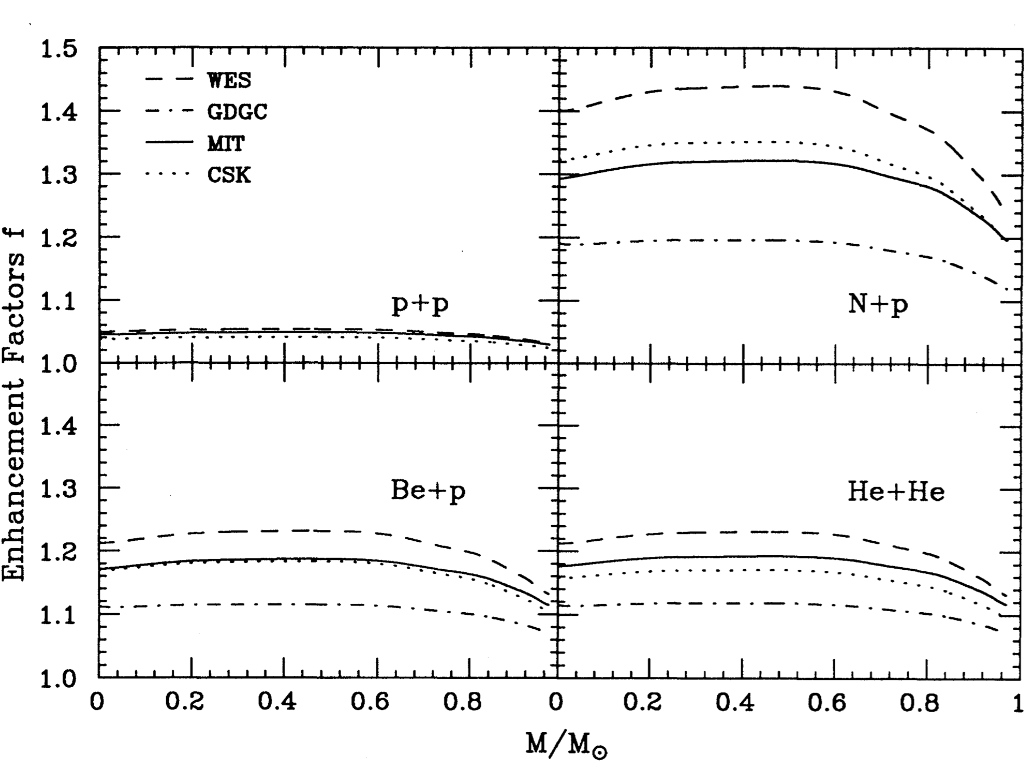
\includegraphics[width=0.4\textwidth,keepaspectratio]{Rscreening}
       \caption{Andamento della correzione di schermaggio degli elettroni secondo diversi schemi. Da \cite{ricci1995screening}.}
\end{wrapfigure}

\begin{comment}
\begin{wraptable}[10]{r}{0.4\textwidth}\label{wrap-tab:escreening}
\pgfplotstabletypeset[
every head row/.style={
 before row={\toprule
 %&\multicolumn{4}{c|}{Primordiale}
 },
 every last row/.style={after row=\bottomrule},
 after row={\midrule}
},
every last row/.style={after row=\bottomrule},
every first column/.style={column type/.add={|}{}},
every last column/.style={column type/.add={}{|}},
%columns/0/.style = {column type/.add={|}{}},
display columns/0/.style={column name={}},
display columns/1/.style={column name={GB}},
display columns/2/.style={column name={GDGC}},
display columns/3/.style={column name={SVH}},
display columns/4/.style={column name={DTDL}},
create on use/react/.style={create col/set list={
$p+p$,$\cel{He}{3}{}{}+\cel{He}{4}{}{}$,$p+\cel{N}{14}{}{}$,$p+\cel{Be}{7}{}{}$}},
columns/react/.style = {column type/.add={|}{}},
columns/react/.style = {column type/.add={}{|}},
columns/react/.style={string type},
columns={react,GB,GDGC,SVH,DTDI},
/pgf/number format/precision=4
     ]{deltaSalpeter.txt} %%%
     \caption{Discrepanze del fattore di screening determinato da diversi autori (vedi \cite{}) $\exp{\Lambda+\delta\Lambda}$ con $\Lambda$ ricavato da Salpeter secondo lo schema accennato: i valori sono $-\delta\Lambda(\%)$.}
\end{wraptable}
\end{comment}

\begin{errata}[Salpeter 1954]
L'energia di interazione di due nuclei $Z_1$ e $Z_2$ a distanza r contiene un contributo delle altre cariche presenti nel plasma:
\begin{equation}
U_T=\frac{Z_1Z_2e^2}{r}+U(r_{12})=Z_1Z_2e^2\psi_T
\end{equation}
dove $U(r_{12})\approx0$ per $r\gg r_D$ e $U(r_{12})\to U_0$ per r che tende a zero; dato che $E_G\gg U_0$ approssimo la correzione a \eqref{eq:fusioncrosssection} con il fattore moltiplicativo
\begin{equation}
f=\exp{-\midfrac{U_0}{KT}}\label{eq:screeningfactor}
\end{equation}

La distribuzione media di carica del plasma, supposto di atomi completamente ionizzati di carica z, si scrive, usando la formula di Boltzmann per descrivere la perturbazione dovuta a $Z_1$:
\begin{equation}
\rho_c(\vec{r})=(\frac{\rho N_Aze}{A})[\exp{\frac{Z_1ze^2}{KT}\psi_T}-\exp{\frac{Z_1e^2}{KT}\psi_T}]
\end{equation}
dove il primo termine \'e una media sugli ioni del gas diversi da $Z_1$ e $Z_2$  e il secondo sugli elettroni.

La condizione che l'energia elettrostatica di due nuclei distanti $r_D$ sia molto minore dell'energia termica definisce il regime di schermaggio debole e risolvendo l'equazione di Poisson per il potenziale generato da $Z_1$: 
\begin{equation}
\nabla^2[Z_1e\psi_T]=-4\pi\rho_c(r)-4\pi Z_1e\delta^{(3)}(r)
\end{equation}
%E_C'-E=\frac{Z_1Z_2e^2}{r}\exp{-\frac{r}{r_D}}-E\approx\frac{Z_1Z_2e^2}{r}-\frac{Z_1Z_2e^2}{r_D}-E=E_C-E-E_D
si ottiene
\begin{equation}
U_0=-\frac{Z_1Z_2e^2}{r_D}
\end{equation}

\end{errata}

L'energia potenziale dovuta all'interazione di due nuclei $Z_1$ e $Z_2$ a distanza r contiene un contributo delle altre cariche presenti nel plasma:
\begin{equation}
U=\frac{Z_1Z_2e^2}{r}+U_s(r_{12})
\end{equation}
dove il primo termine \'e l'energia potenziale non schermata e il termine $U_s(r_{12})$ il contributo della nuvola elettronica. L'effetto di $U_s$ \'e di aumentare la probabilit\'a di attraversamento della barriera coulombiana. Correggo quindi \eqref{eq:fusioncrosssection} con il fattore moltiplicativo:
\begin{equation}
f=\exp{-\midfrac{U_0}{KT}}\label{eq:screeningfactor}
\end{equation}
dove $U_0=U_s(0)$ poich\'e $r\ll r_D$ e considerando solo la correzione al fattore di penetrazione ($E_G\gg U_0$).

Per determinare $U_0$ considero l'energia potenziale di $Z_1$ e $Z_2$ a distanza $r$
\begin{equation}
U=Z_2e\int_{\infty}^r\PDy{r_1}{\phi_1}\,dr_1=\frac{Z_1Z_2e^2\exp{-\midfrac{r}{r_D}}}{r}
\end{equation}
con $\phi_1$ dato da \eqref{eq:screenedpotential}, e quindi
\begin{equation}
U_s=U-\frac{Z_1Z_2e^2}{r}
\end{equation}

Sulla base dell'efficienza delle reazioni nucleari, del profilo di densit\'a e temperatura ricavati da un modello solare le terminazione della catena pp $\cel{He}{3}{}{}-\cel{He}{3}{}{}$ e $\cel{He}{3}{}{}-\cel{He}{4}{}{}$ generano rispettivamente $83.3\%$, $16.7\%$ della luminosit\'a totale mentre il ciclo CNO circa $1\%$.
%\begin{wrapfigure}[23]{r}{0.6\textwidth}
% T_6=10T_7=10^3T_9
\thispagestyle{plain}

{\let\clearpage\relax\let\cleardoublepage\relax
\chapter{Modello solare standard e osservabili sismologiche.}
}

\begin{figure}[!h]
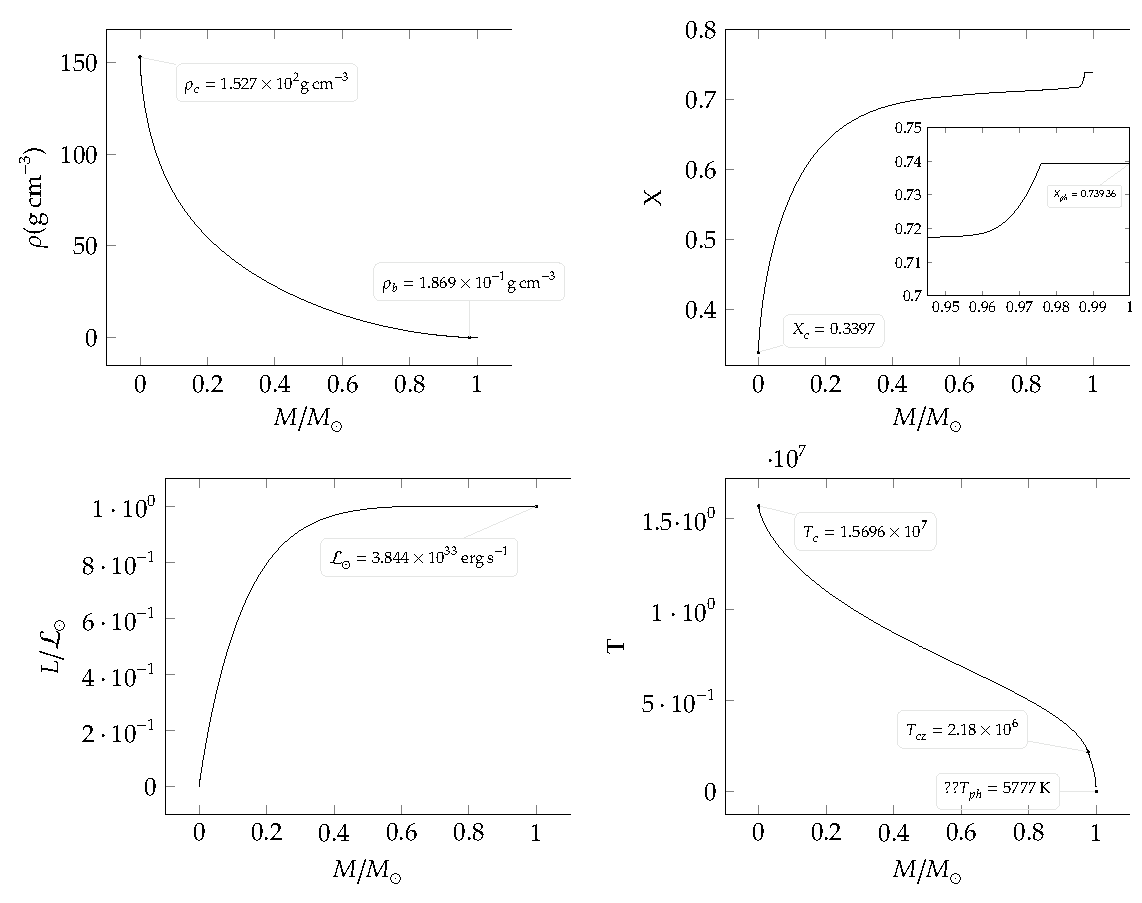
\includegraphics[width=\textwidth,trim=4 4 4 4,clip]{BP2000}
\caption{Profilo radiale della densit\'a, abbondanza di idrogeno, luminosit\'a e temperatura; sono indicati i valori centrali e alla base della zona convettiva. Dati da \cite{BP2000}.}
\end{figure}

\begin{workout}[modellizzazione della fisica del plasma solare/accuratezza]
La modellizzazione della fisica del plasma solare (EOS, opacit\'a,) sono necessarie approssimazioni che ne influenzano l'accuratezza, 
\end{workout}

\begin{workout}[e incertezze in Z]

\end{workout}

%La composizione determinata usando righe di assorbimento dell'atmosfera  poich\'e l'assorbimento continuo \'e dovuto principalmente all'idrogeno l'abbondanza degli elementi pesanti si esprime relativamente all'abbondanza di idrogeno.
%Modelli di atmosfera pi\'u accurati, possibili grazie a maggiore potenza di calcolo, hanno fornito composizione di metalli sensibilmente minore

Determino la struttura solare integrando numericamente le equazioni fondamentali della struttura stellare
\begin{subequations}\label{subeqn:stellarstructure}
\begin{align}
&\TDy{r}{m}=4\pi r^2\rho\\
&\TDy{r}{P}=-\frac{Gm(r)\rho(r)}{r^2}\\
&\TDy{r}{T}=\nabla\frac{T}{p}\TDy{r}{p}\\
&\TDy{r}{L}=4\pi r^2[\rho(\epsilon-\epsilon_{\nu})-\rho\TDof{t}u+\frac{P}{\rho}\TDy{t}{\rho}]
\end{align}

\begin{equation}
\PDy{t}{n_i}+\frac{1}{r^2}\PDof{r}(r^2n_iv_i)=\Dcvar{\PDy{t}{n_i}}{Nucl}\label{eq:difffusionchange}
\end{equation}
\end{subequations}
con $v_i$ velocit\'a di diffusione specie i. Ottengo il profilo radiale delle grandezze $\{P,m,T,L,X_i\}$, note la metallicit\'a iniziale Z, l'equazione di stato $P(\rho,T,X_i)$, l'opacit\'a $\kappa(P,T,X_i)$, il rate di produzione di energia nucleare per grammo $\epsilon(P,T,X_i)$.

Le condizioni al bordo per le equazioni precedenti sono:
\begin{itemize}
    \item La superficie \'e definita da $T=T_{eff}$ e si ha la condizione $\lsun{}=4\pi r^2\sigma T_{eff}^4$. La pressione alla superficie \'e legata alla struttura di equilibrio dell'atmosfera.

    \item In $r=0$ deve essere $L=0$, $M=0$.
    %e condizioni al centro si ricavano espandendo l, m attorno a $r=0$ in termini di $T_c, P_C,X_C,X_{3C}$ ed eguagliando le espansioni ai valori di l e m del punto pi\'u interno.
\end{itemize}

Per determinare il modello solare attuale evolvo il modello del Sole in sequenza principale partendo da una composizione chimica fissata fino ad ottenere un modello con le caratteristiche del Sole attuale:
\begin{itemize}
\item Il valore di Y \'e determinato dalla luminosit\'a solare attuale: l'aumento del peso molecolare medio $\mu$, determinato tramite \eqref{eq:difffusionchange}, dovuto principalmente alle reazioni di fusione \eqref{eq:energyrate}, deve essere compensato da un'aumento di temperatura con conseguente incremento dell'energia generata e della luminosit\'a.

\item L'efficienza della convezione determina il gradiente della regione esterna convettiva \'e scelta in maniera da avere la temperatura efficace attuale, cio\'e il raggio attuale; in generale devo  fare ulteriore correzione perch\'e cambiando il gradiente termico della regione esterna la soluzione delle equazioni stellari avr\'a in generale un profilo termico leggermente diverso e un modello solare che non riproduce la luminosit\'a attuale.

\item La composizione iniziale \'e determinata in maniera da riprodurre quella attuale tenendo conto della diffusione.
\end{itemize}


%\begin{workout}[Reaction rates]
%\begin{wrapfigure}[10]{r}{0.5\textwidth}
       %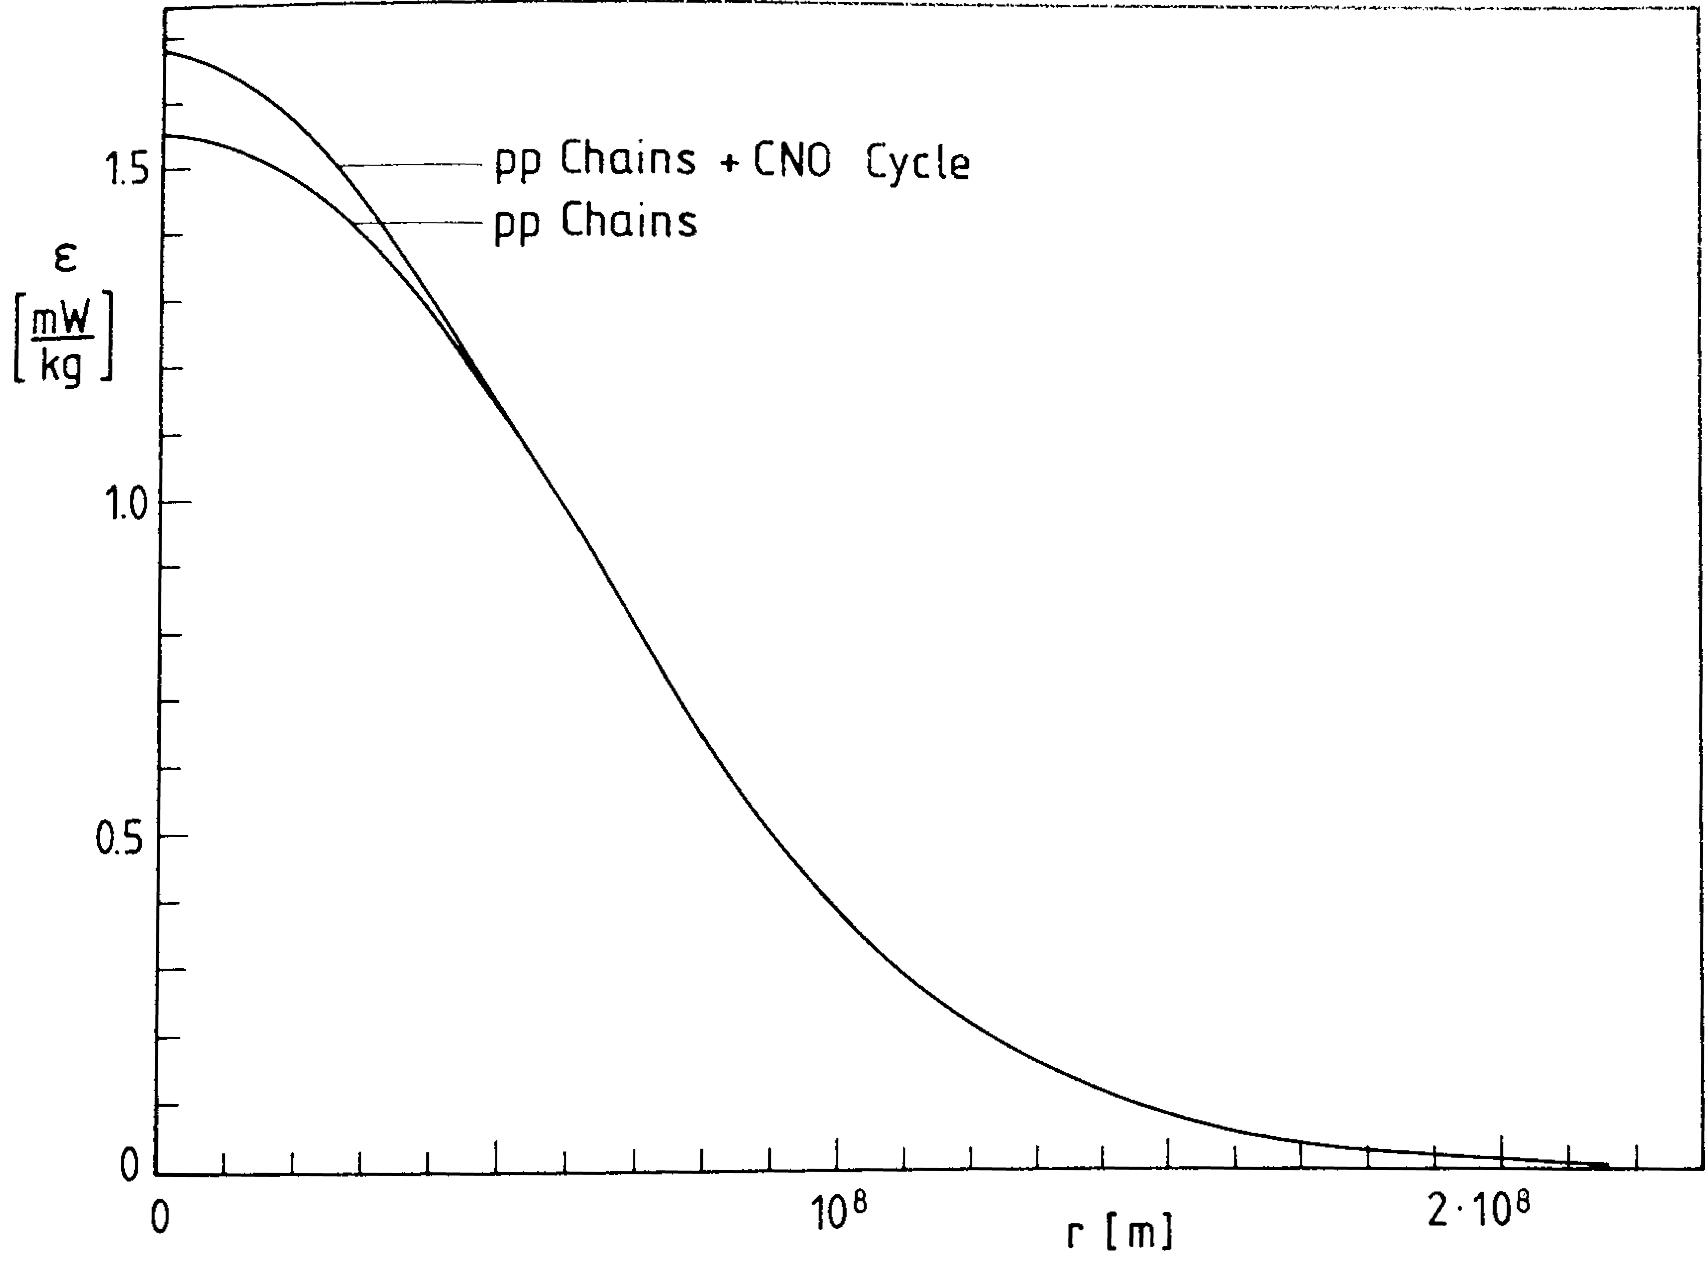
\includegraphics[width=0.45\textwidth,keepaspectratio]{watt-PPvsCNO}
        %\caption{Andamento dell'energia generata per unit\'a di massa nel Sole: il contributo della catena PP \'e dominante rispetto ad altre reazioni.}

%\clearpage

\section{Caratteristiche solari determinate dall'eliosismologia}

L'osservazione della superficie solare ha rivelato la presenza di oscillazioni descrivibili come modi normali adiabatici dell'intera struttura solare determinati da $P(r)$, $\rho(r)$, $g(r)$ e $\Gamma_1(r)$: poich\'e queste quantit\'a sono legate dalle equazioni della struttura stellare si considerano 2 combinazioni indipendentidi queste grandezze. La quantit\'a fondamentale determinata dalla misura delle frequenze dei modi, data la natura prevalentemente acustica, \'e
\begin{equation}
c_s^2=\Gamma_1\frac{P}{\rho}
\end{equation}

\begin{figure}[!ht]
\begin{subfigure}[r]{0.5\textwidth}
        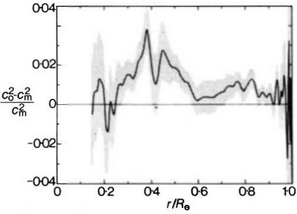
\includegraphics[width=0.99\textwidth,keepaspectratio]{dsoundspeedduvall}
        \caption{Differenza relativa del profilo di $c_s$ (determinata invertendo \eqref{eq:analinversionc}) per frequenze dei modi calcolate con MSS e osservate. La differenza relativa \'e minore del $5\%$. Da \cite{christensen1985speed}.}
\label{dsoundduvall}
    \end{subfigure}
~
\begin{subfigure}[r]{0.5\textwidth}
        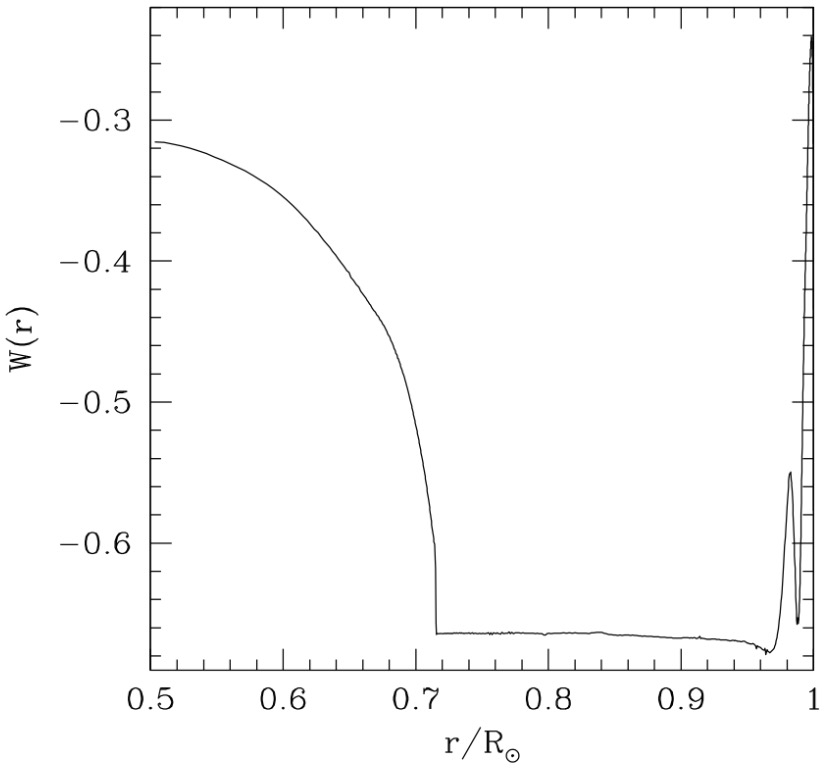
\includegraphics[width=0.99\textwidth,keepaspectratio]{WrbczHHeioniz}
        \caption{Profilo di W calcolato da un modello solare. Da \cite{basu2008helioseismology}.}\label{fig:dlessc}
    \end{subfigure}
\end{figure}

La regione radiativa ha stratificazione sub-adiabatica mentre a partire da $r=R_b$ si ha stratificazione quasi-adiabatica,  $\Gamma_1\approx\frac{5}{3}$: $P\propto\rho\expy{\frac{5}{3}}$. Il gradiente adimensionale della velocit\'a del suono $W$ mette in risalto la discontinuit\'a del gradiente termico (alla base della zona convettiva) e in $\Gamma_1$ (nelle zone di ionizzazione):
\begin{equation}
W=\frac{1}{g}\TDy{r}{c^2}%=\Gamma_1(\invers{\PDly{\rho}{P}}-1)
\end{equation}



Nella figure (\subref{fig:dlessc}) si vedono la base della zona convettiva intorno a $0.7\rsun{}$ e i picchi dovuti alle regioni di ionizzazione a $HeII$, intorno a $0.98\rsun{}$, e di ionizzazione di $HI$ e $HeI$ verso la superficie: \'e possibile determinare l'abbondanza di $He$ nella zona convettiva anche se non \'e la tecnica pi\'u accurata.

Il buon accordo tra il profilo di $c_s$ determinato eliosismologicamente e calcolato da un modello solare (\subref{dsoundduvall}) giustifica l'uso del modello per calcolare il comportamento dei modi solari che come illustrer\'o nell'ultima parte permette di determinare il profilo di $\rho$ e $c_s$ in miglior accordo con le osservazioni.

\begin{wrapfigure}[15]{r}{0.5\textwidth}
        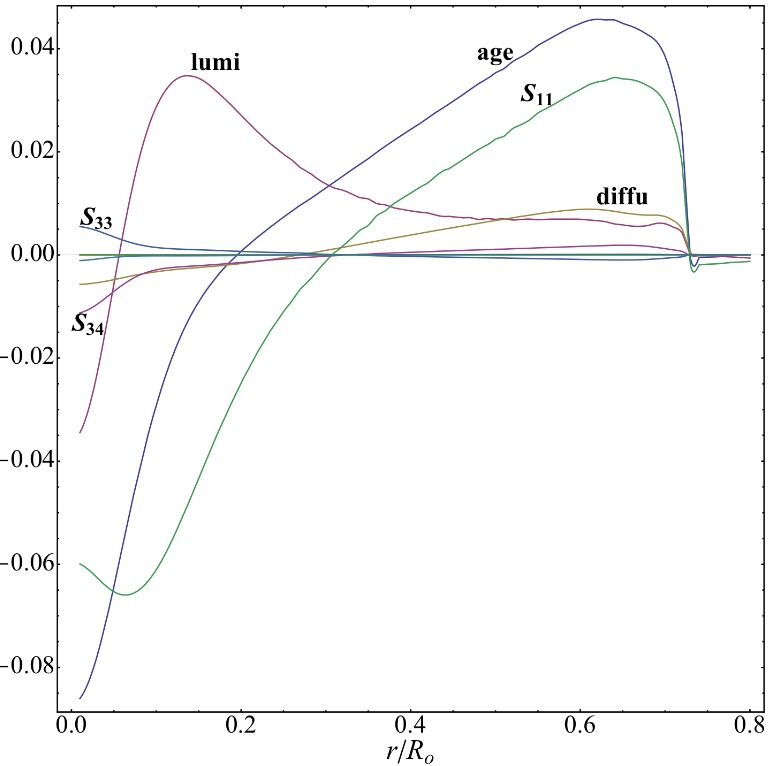
\includegraphics[width=0.5\textwidth,keepaspectratio]{deltaCdeltaQ}
        \caption{Profilo della derivata logaritmica di $c_s$ rispetto ai parametri del MSS $(\PDly{Q}{c_s})$. Da \cite{villante2014chemical}.}
\end{wrapfigure}

Inoltre ricavando da un modello solare la dipendenza delle quantit\'a determinate eliosismicamente dai parametri del modello \'e possibile imporre dei vincoli ai parametri cercando i valori dei parametri che meglio riproduco le grandezze determinate eliosismologicamente.


%dlncdlnzjdetailed}
        %\caption{Derivata della velocit\'a del suono rispetto a $z_i=\midfrac{Z_{ph}}{x_{ph}}$. Da \cite{villante2014chemical}.}




\end{document}